\documentclass[letterpaper,landscape]{slides}
%\documentclass[letterpaper,portrait]{slides}
\usepackage{boxedminipage}

%\input /u/rhl/TeX/pdf.tex
\input pdf.tex

\newif\ifTalk\Talktrue		% We generating a talk, not printing
%\Talkfalse			% no; we're really printing

%\pagestyle{empty}
\setlength{\topmargin}{-1in}
\setlength{\textheight}{7.5in}
\setlength{\textwidth}{9in}
\setlength{\oddsidemargin}{0pt}
\setlength{\oddsidemargin}{0pt}

%\onlyslides{1-3,4,10-9999}
%\onlyslides{26-9999}

\begin{document}

\newcommand{\XXX}[1]{\textbf{XXX} #1}
\newcommand{\colour}[1]{\color{#1}}


\def\eq#1{\begin{equation} \color{blue} #1 \end{equation}}
\def\vx{{\bf x}}
\def\vv{{\bf v}}
\def\b#1{{\bf  #1}}
\def\p{\partial}
\def\th{^{th}}
\def\msun{{\rm\,M_\odot}}
\def\bnabla{{\bf\nabla}}
\def\dint{\int\!\!\!\int}
\def\d{{\rm d}}
\def\i{{\rm i}}
\def\ddt#1{{\rm{d} #1\over {\rm dt}}}
\def\ddtS#1{{\rm{d^2} #1\over {\rm dt^2}}}
%\lta and \gta produce > and < signs with twiddle underneath
\def\spose#1{\hbox to 0pt{#1\hss}}
\def\lta{\mathrel{\spose{\lower 3pt\hbox{$\mathchar"218$}}
     \raise 2.0pt\hbox{$\mathchar"13C$}}}
\def\gta{\mathrel{\spose{\lower 3pt\hbox{$\mathchar"218$}}
     \raise 2.0pt\hbox{$\mathchar"13E$}}}
\def\mspace{\hbox{\quad}}

\def\deffn#1{{\bf#1}}\def\eqs#1{equations \rf#1}


\newcount\itemCnt\itemCnt=0
\newcommand{\nitem}{%
  \global\advance\itemCnt by 1
  ~\vskip0cm\the\itemCnt.\qquad}

\definecolor{orange}{rgb}{1.0, 0.5, 0.0}
\definecolor{purple}{cmyk}{0.4, 0.8, 0.3, 0.0}


%%%%%%%%%%%%%%%%%%%%%%%%%%%%%%%%%%%
\newcommand{\onepic}[6]{%
\begin{slide}
     \begin{center}
        \begin{minipage}{#1in}
            {\large \color{blue} #6}
            \phantom{x} \vskip #2in
            \phantom{x} \hskip #3in
            {\scalebox{#4}{\includegraphics{#5}}}   
        \end{minipage}
     \end{center}
    \vfill
\end{slide}
}


%%%%%%%%%%%%%%%%%%%%%%%%%%%%%%%%%%%
\newcommand{\picslide}[7]{%
  \begin{slide}
     \begin{center}
        \begin{minipage}{#5in}
            \hskip #6in
            \hskip -1in
            {\scalebox{#4}{\includegraphics{#1.#2}}}
            \vskip #7in~
            {\large \color{blue} #3}
        \end{minipage}
     \end{center}
     \vfill
  \end{slide}
}
%%%%%%%%%%%%%%%%%%%%%%%%%%%%%%%%%%%
 

%%%%%%%%%%%%%%%%%%%%%%%%%%%%%%%%%%%
\newcommand{\Spicslide}[7]{%
  \begin{slide}
     \begin{center}
        \begin{minipage}{#5in}
            \vskip #6in
            \hskip #7in
            {\scalebox{#4}{\includegraphics{#1.#2}}}
        \end{minipage}
     \end{center}
     \vfill
  \end{slide}
}
%%%%%%%%%%%%%%%%%%%%%%%%%%%%%%%%%%%
 


%------------------------------------------------------------------------------
%------------------------------------------------------------------------------

\begin{slide}

\phantom{x}
\vskip -2in
\begin{center}
\bfseries
{\large {\color{blue} Astr 511: Galaxies as galaxies}}
\end{center}

{\centerline {{\color{blue} 
Winter Quarter 2017, University of Washington}}}
{\centerline {{\color{blue} 
Mario Juri\'{c} \& \v{Z}eljko Ivezi\'{c} }}}

\vskip 1.6in

{\centerline {\huge {\color{red}      Lecture 13:             }}}
\vskip 0.2in 
{\centerline {\Large {\color{blue}  Stellar metallicity and kinematics in the Milky Way }}}

\vfill
\end{slide}
%------------------------------------------------------------------------------



%------------------------------------------------------------------------------
% TWO-SIDED PAGE 
\begin{slide}

\hbox to \hsize{
\begin{minipage}[t]{16cm}
\begin{center}
\vskip -1.7in
\scalebox{0.4}{\hskip -3.3in 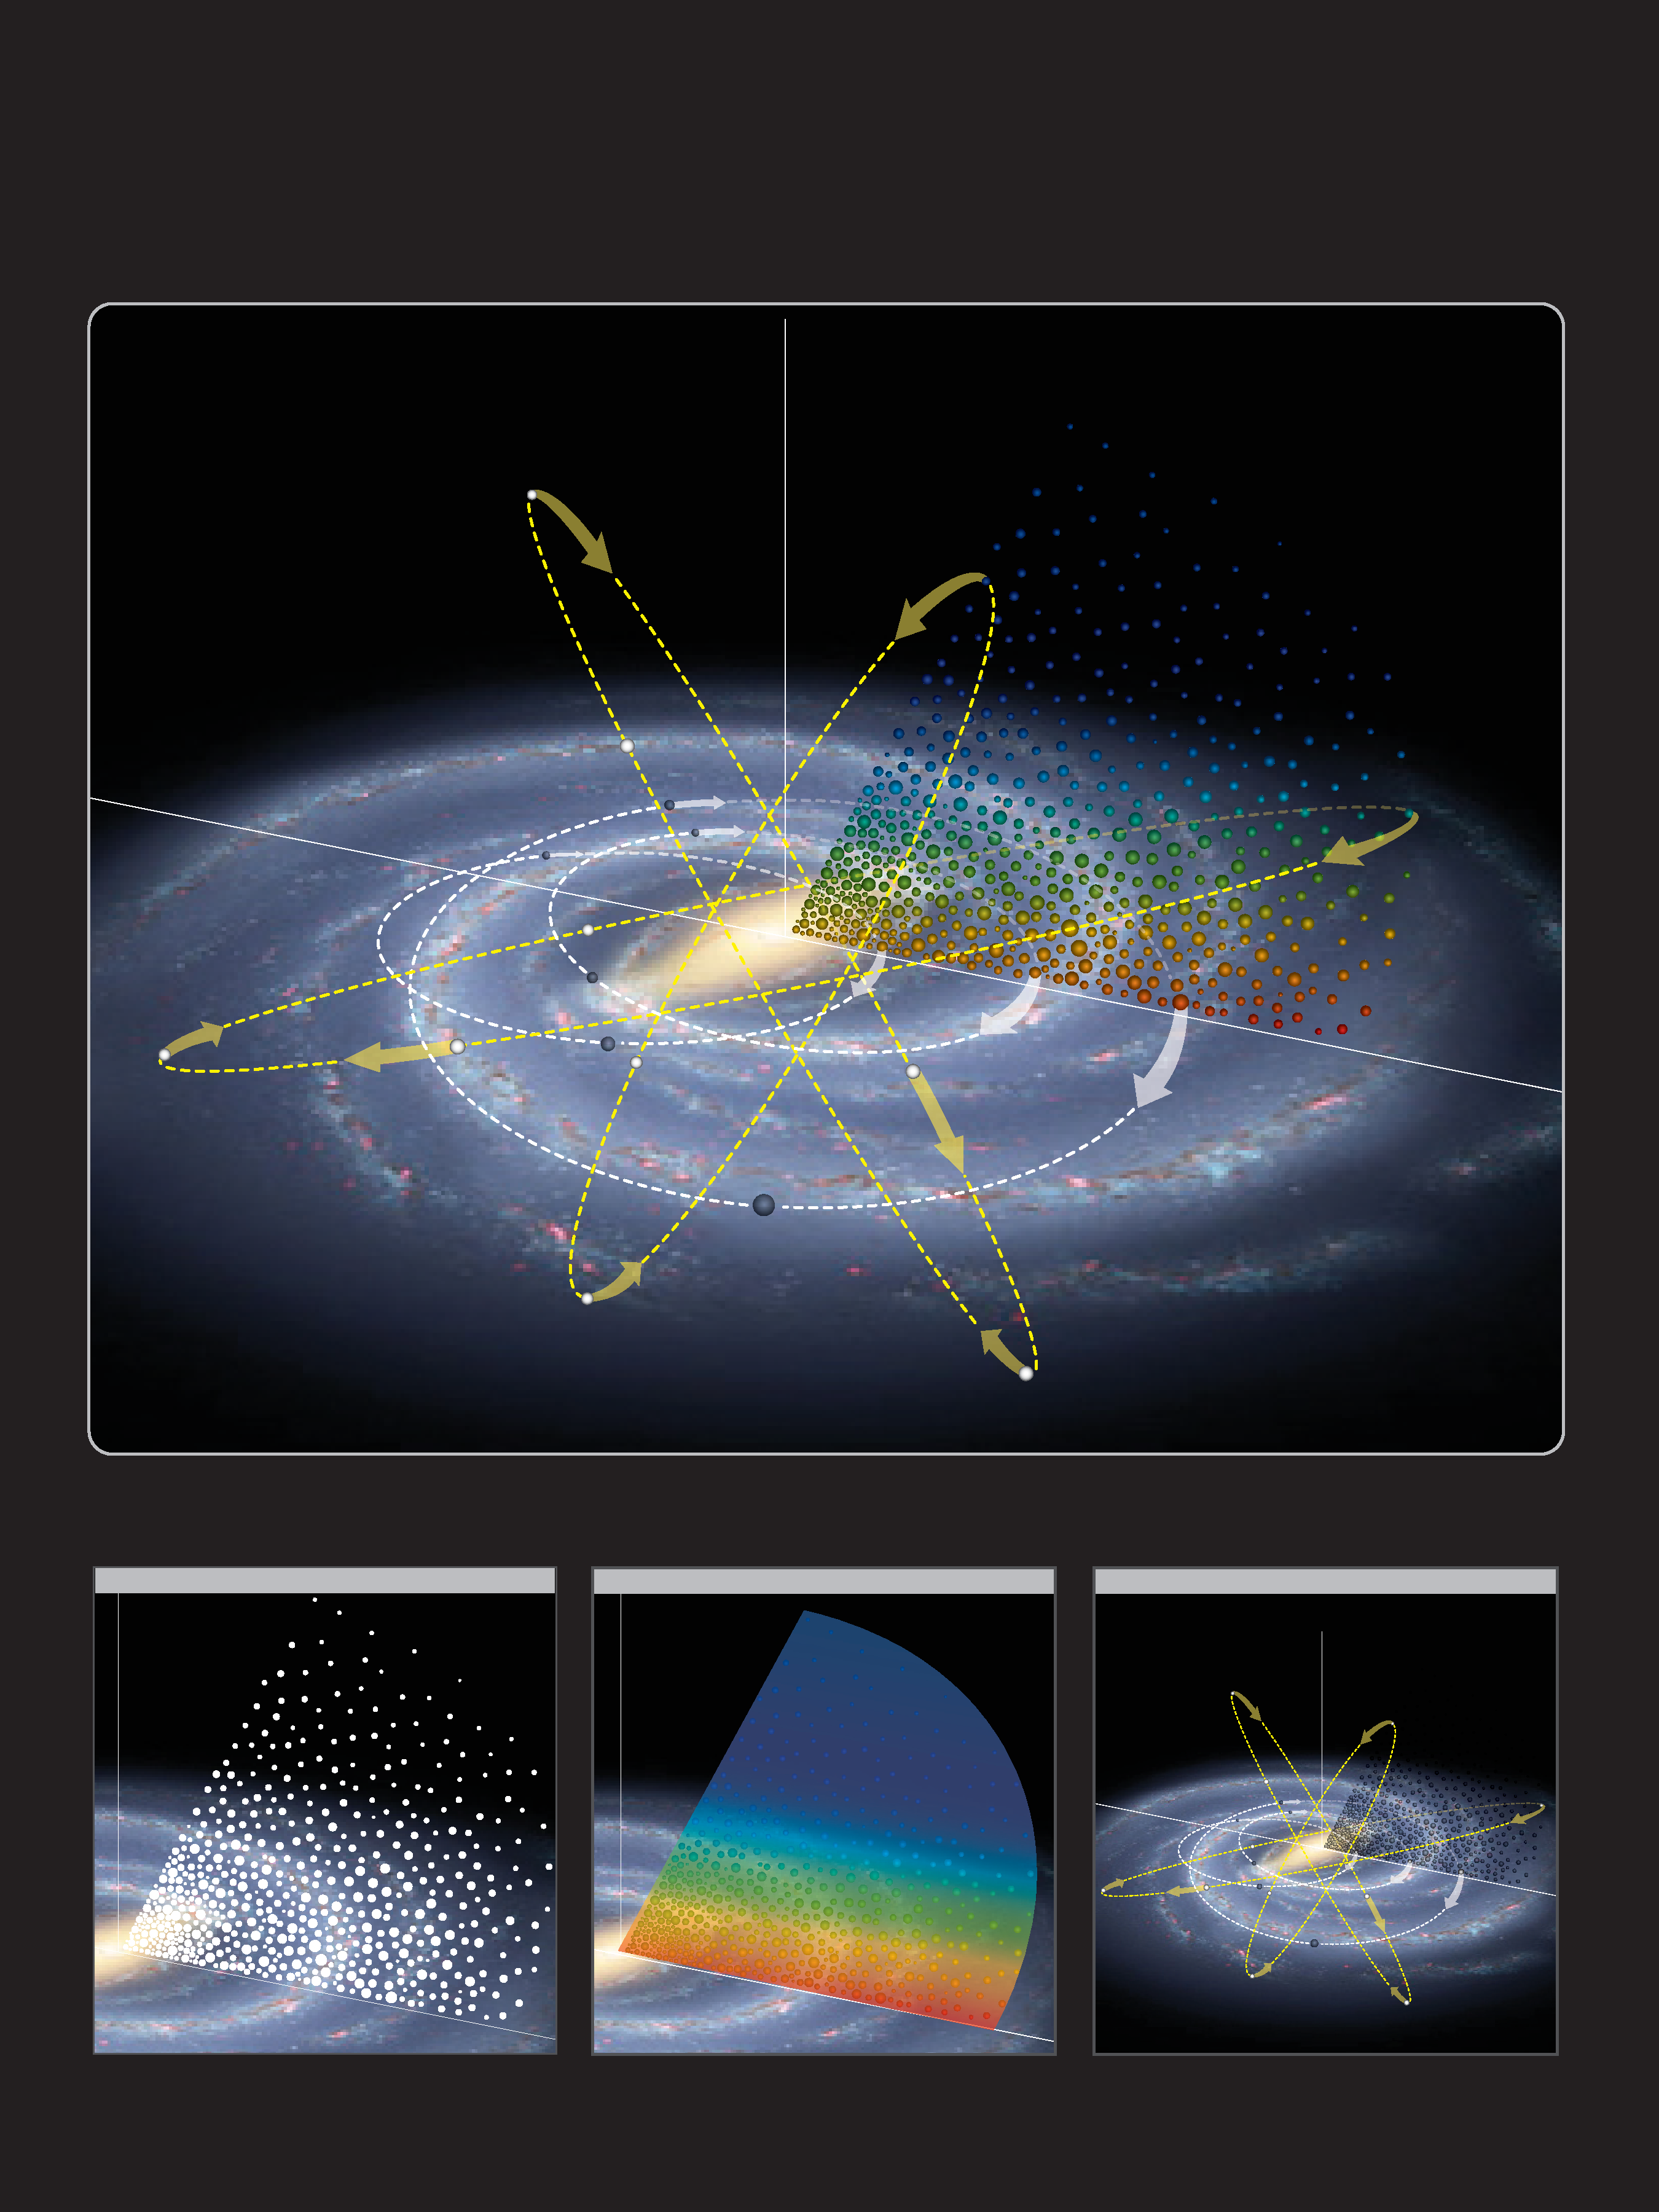
\includegraphics{figures/MW_Poster18x24_noText.pdf}}

\end{center}

\end{minipage}

\begin{minipage}[t]{8cm}
\begin{center}
{\large \color{red} The three basic stellar distribution functions:}
\end{center}
\vskip 0.3in
\begin{enumerate}
\item {\bf Number density}
\item  {\bf Metallicity}
\item  {\bf Kinematics} 
\end{enumerate}     

{\large \color{blue} These three distribution functions provide
observational constraints for the model selection} (models for
galaxy formation and evolution)


\end{minipage}}
\vfill 
\end{slide}
%------------------------------------------------------------------------------


%------------------------------------------------------------------------------
\begin{slide}
\begin{center}
\bfseries
{\large {\color{blue} Outline} }
\end{center}
\vskip -1.2in

\begin{enumerate}
            \item {\bf Metallicity distribution: introduction, disk vs. halo}
             \item {\bf Stellar Kinematics: measurements}
             \item {\bf Stellar Kinematics: disk vs. halo}
\end{enumerate}
\vskip -0.3in
{\color{red} \bf Reading:}
\vskip -0.3in
   \begin{itemize}
   \item {\color{blue} Ivezi\'{c} et al. 2008 (ApJ 684, 287):} Sec. 3.4 and 4 at least
   \item {\color{blue} Bond et al. 2010 (ApJ 716, 1):} Sec. 1 to 6 at least 
   %\item {Carollo et al. 2010 (ApJ 712, 692):} Sec. 1 and 11 at least 
   \item {Reid \& Hawley:} ch. 7 and 8; {Binney \& Merrifield:} ch. 10
\end{itemize}


\vfill
\end{slide}
 
%------------------------------------------------------------------------------



%------------------------------------------------------------------------------

\begin{slide}
\begin{center}
{\large \color{red} Introduction: metallicity}
\end{center}

\begin{itemize}
\item
Given the {\color{red} mass fraction} of hydrogen, $X$, and the fraction of helium $Y$, the fraction of all the remaining chemical 
elements is $Z = 1 - X - Y$. 
\item 
For the Sun, $X_\odot=0.7381$, $Y_\odot=0.2485$ and $Z_\odot = 0.0134$
(Asplund et al. 2009, ARA\&A 47, 481). 
\item Metallicity is defined, using {\color{red} {\it the numbers of atoms}}, as \\
   $ [Fe/H] = \log_{10}\left( N_{Fe} / N_H \right)_{\ast} - \log_{10}\left( N_{Fe} / N_H \right)_\odot$. 
\item 
The following proportionality is usually assumed, with $C\sim 1$ (to within 10\% or so), \\
$ [M/H] \equiv \log_{10}\left({ Z_\ast/X_\ast \over Z_\odot / X_\odot }\right)  = C \, [Fe/H]$. 
\item Confusingly, both $[M/H]$ and $[Fe/H]$ are called ``metallicity''. 
\end{itemize}  


\vfill
\end{slide}
%------------------------------------------------------------------------------


%------------------------------------------------------------------------------
% TWO-SIDED PAGE 
\begin{slide}

\hbox to \hsize{
\begin{minipage}[t]{12cm}
\begin{center}
\vskip 0.2in 
\scalebox{0.7}{\hskip -1.4in 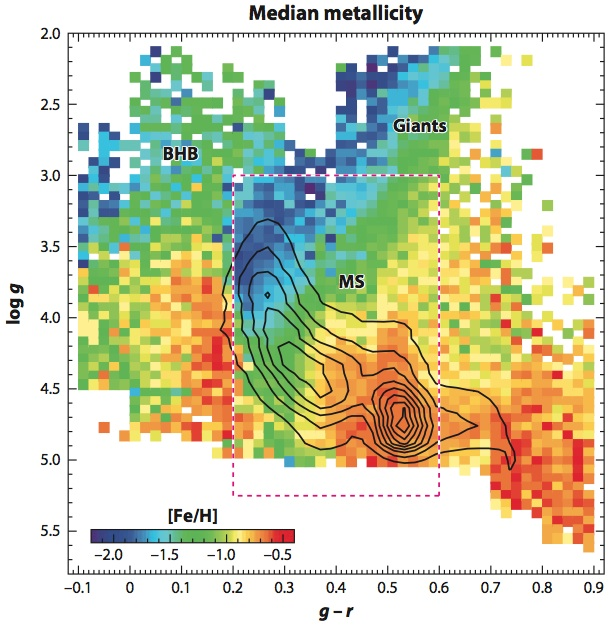
\includegraphics{figures/IBJ2012_fig1.jpg}}
\end{center}
\end{minipage}


\begin{minipage}[t]{12cm}
\begin{center}
\vskip -1in
{\large \color{red} Stellar Parameters Estimation}
\end{center}
\begin{itemize}
\item SDSS stellar spectra are automatically processed to obtain stellar 
       parameters such as {\bf effective temperature, gravity, metallicity}. 
\item {\bf Left:} resembles a warped HR diagram; the color-coded map shows
     the median metallicity as a function of $log(g)$ (roughly, dwarfs vs. giants)
     and the $g-r$ color (roughly, effective temperature), according to the 
     legend in the bottom left corner; the contours show
     the distribution of all SDSS stars with spectra (biased!)
\end{itemize} 
\end{minipage}}
\vfill 
\end{slide}
%-----------------------------------------------------------------------------


% Rosalie's low-FeH vs high-FeH comparison
\Spicslide{figures/rosalieS23compare2}{jpg}{}{0.9}{7}{0.3}{-1.5} 


%------------------------------------------------------------------------------
% TWO-SIDED PAGE 
\begin{slide}

\hbox to \hsize{
\begin{minipage}[t]{8cm}
\begin{center}
\vskip -0.7in 
\scalebox{0.75}{\hskip -1.4in 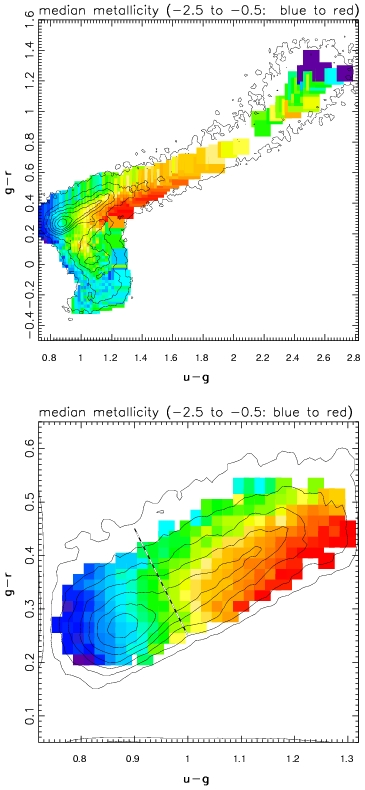
\includegraphics{figures/params_ugr_metal.jpg}}
\end{center}
\end{minipage}


\begin{minipage}[t]{16cm}
\begin{center}
\vskip -1in
{\large \color{red} Stellar Parameters Estimation: $[Fe/H]$}
\end{center}
\begin{itemize}
\item {\color{blue} Stellar parameters estimated from spectra show a good correlation with
      colors measured from imaging data}
\item {\bf Top left:} the median metallicity as a function of 
     the position in the $g-r$ vs. $u-g$ diagram  ($-$0.5 to $-$2.5, red to blue)
\item {\bf Bottom left:} zoomed-in version of the top left figure
\item {\color{blue} Photometric estimate of metallicity:} can be determined with 
      an error of $\sim$0.2-0.3 dex (relative to spectroscopic estimate) from the position 
      in the $g-r$ vs. $u-g$ color-color diagram using simple expressions
\item {\color{red} This finding is important for studies based on photometric data alone, and also
      demonstrates the robustness of parameters estimated from spectroscopic data}
\end{itemize} 
\end{minipage}}
\vfill 
\end{slide}
%-----------------------------------------------------------------------------

% from TomoIII
\Spicslide{figures/QAphotoFeH}{jpg}{}{0.9}{7}{0.0}{-1.0} 


%------------------------------------------------------------------------------
% TWO-SIDED PAGE 
\begin{slide}

\hbox to \hsize{
\begin{minipage}[t]{13cm}
\begin{center}
\vskip -0.5in
\scalebox{0.7}{\hskip -1.5in 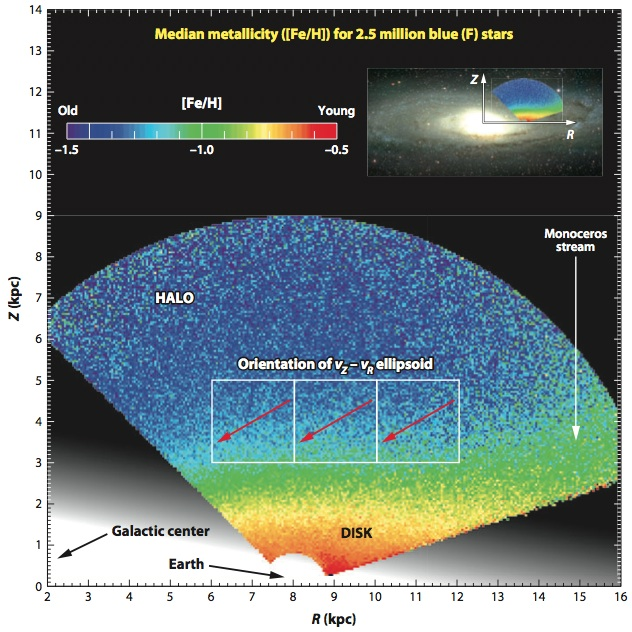
\includegraphics{figures/IBJ2012_fig5.jpg}}

{\bf A harder analysis problem than counts; instead of a single
count value, at each position there is a (scalar) distribution function,
p([Fe/H])!}


\end{center}
\end{minipage}

\begin{minipage}[t]{10cm}
\begin{center}
\vskip -1in
{\large \color{red} Photometric Metallicity Distribution}
\end{center}

\begin{itemize}
\item {\color{blue} Panoramic view of the Milky Way metallicity distribution:}
the median metallicity map contains $\sim$8,000 pixels (0.1 kpc by 0.1
kpc), and is based on a complete flux- and color-limited sample of $\sim$2.5 
million blue stars. 
\item {\color{blue} The median metallicity is a strong function of distance
from the Galactic plane;} deviations are associated with spatial (and
kinematic) substructures
\end{itemize}     

\end{minipage}}
\vfill 
\end{slide}
%------------------------------------------------------------------------------


%------------------------------------------------------------------------------
% TWO-SIDED PAGE 
\begin{slide}

\hbox to \hsize{
\begin{minipage}[t]{6cm}
\begin{center}
\vskip -0.8in
\scalebox{1.0}{\hskip -0.7in 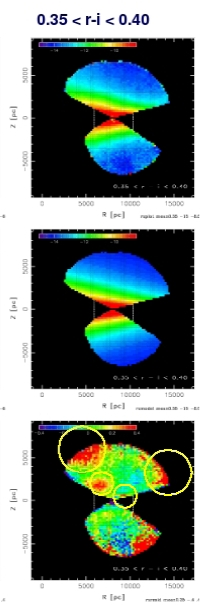
\includegraphics{figures/J08counts.jpg}}
\vskip -2.6in
\scalebox{0.46}{\hskip -1.8in 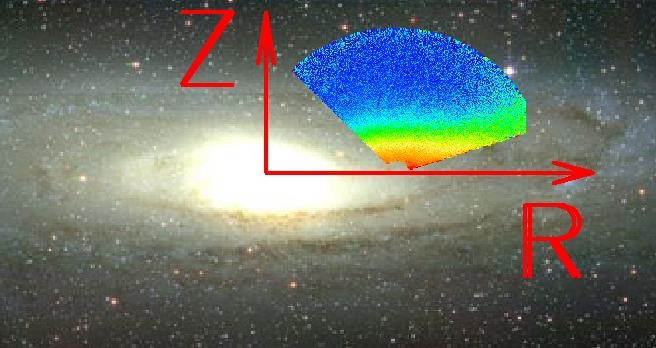
\includegraphics{figures/coordEx.jpg}}
\vskip -1.42in 
{\color{blue} \hskip 1.04in \bf o}
\end{center}
\end{minipage}

\begin{minipage}[t]{17cm}
\begin{center}
\vskip -1in
{\large \color{red} Dissecting the Milky Way with SDSS }
\end{center}

\begin{itemize}
\item {\color{blue} Panoramic view} of the Milky Way, akin to observations 
of external galaxies; {\color{blue} good support for standard Galactic models}
(with amazing signal-to-noise!)
\item
{\color{red} Metallicity mapping} supports components inferred 
from number counts mapping
\end{itemize}     

\vskip 0.05in
\scalebox{0.55}{\hskip 1.6in 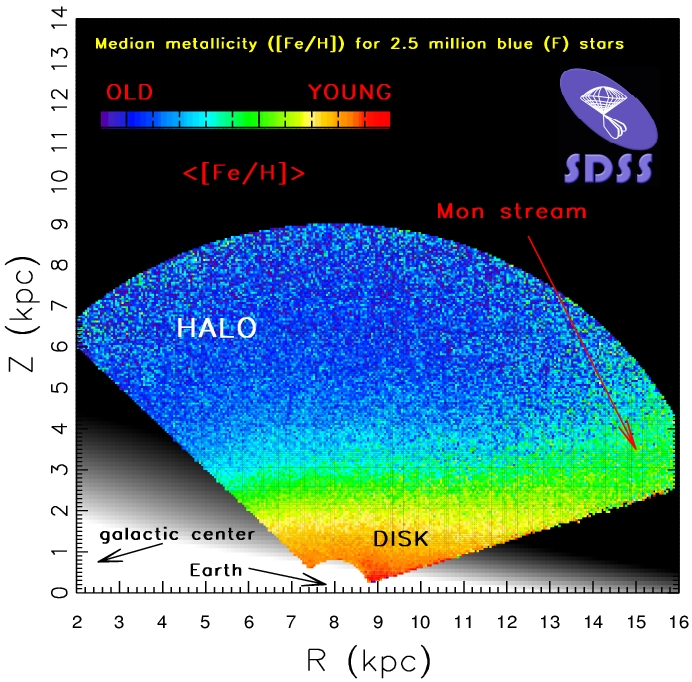
\includegraphics{figures/FeHpress.jpg}}

\end{minipage}}
\vfill 
\end{slide}
%------------------------------------------------------------------------------



% from TomoIII
\Spicslide{figures/FeHmodels}{jpg}{}{0.9}{7}{0.0}{-1.0} 
%------------------------------------------------------------------------------





%------------------------------------------------------------------------------
% TWO-SIDED PAGE 
\begin{slide}

\hbox to \hsize{
\begin{minipage}[t]{8cm}
\begin{center}
\vskip -0.8in 
%\scalebox{1.0}{\hskip -1.0in \includegraphics{loebman1.jpg}}
\scalebox{0.8}{\hskip -1.0in 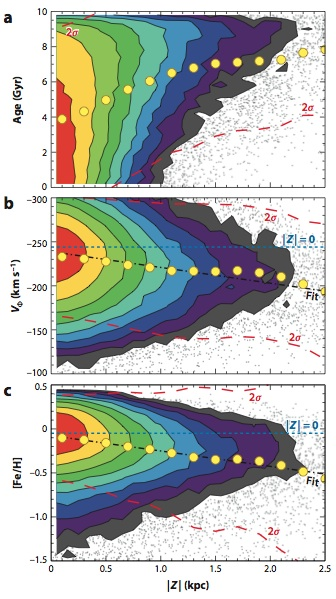
\includegraphics{figures/IBJ2012_fig13.jpg}}
\end{center}
\vskip -0.2in
\leftline{\bf \hskip -1.0in Loebman et al. 2011}
\leftline{\bf \hskip -1.0in (ApJ, 737, 17) }
\leftline{\bf \hskip -1.0in (Ro\v{s}kar et al. models)}
\end{minipage}


\begin{minipage}[t]{16cm}
\vskip -1in
\begin{center}
{\large \color{red}  Is Thin/Thick Disk an Age Effect?}
\end{center}
\begin{itemize}
\item {\color{blue} Data:} Change of slope of stellar counts at $\sim1$ kpc, and both rotational 
velocity distribution and metallicity distribution for disk stars vary with $Z$
\item {\color{blue} {N-body models with radial migration:} \,\,\,\,\, 1) behave like the data, and \\ 2) provide
age information and details about radial migration}  
\item {\color{red} {\bf Models:} Older stars 1) reach larger $|Z|$, 2) have lower [Fe/H], 3) display
rotational velocity lag, 4) no [Fe/H]-$v_\phi$ correlation} {\bf \color{blue} Observers call this behavior ``thick disk''}
\end{itemize} 

\vskip 0.3in
\scalebox{1.3}{\hskip -0.2in \includegraphics{figures/loebman2.jpg}}

\end{minipage}}
\vfill 
\end{slide}
%-----------------------------------------------------------------------------






%------------------------------------------------------------------------------
% TWO-SIDED PAGE 
\begin{slide}

\hbox to \hsize{
\begin{minipage}[t]{15cm}
\begin{center}
\vskip -0.7in
%\scalebox{0.8}{\hskip -1.3in 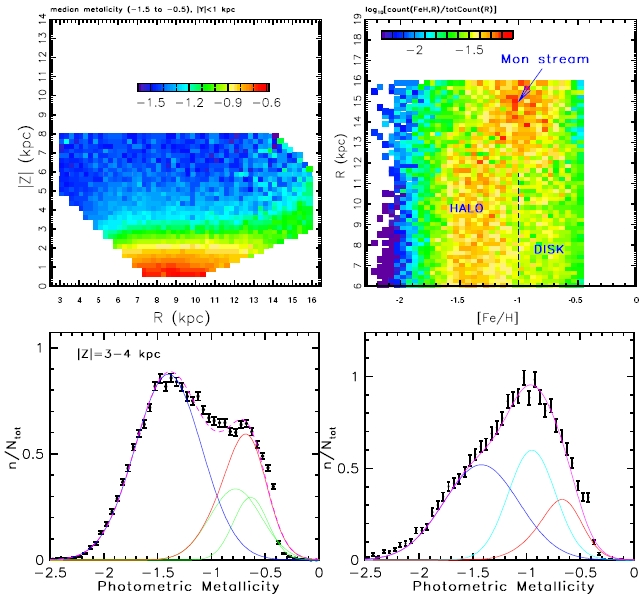
\includegraphics{MonAnalysis.jpg}}
\scalebox{0.8}{\hskip -1.0in 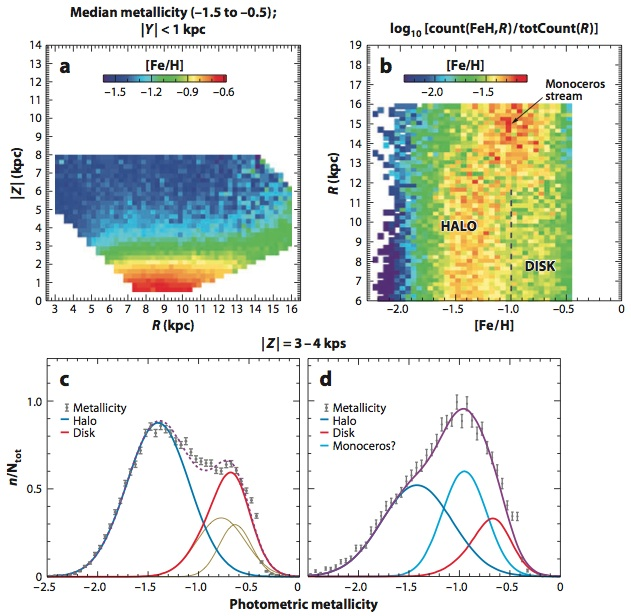
\includegraphics{figures/IBJ2012_fig19.jpg}}

{\bf  There is fine substructure in the metallicity distribution!}

\end{center}
\end{minipage}

\begin{minipage}[t]{8cm}
\begin{center}
\vskip -1in
{\large \color{red} \,\,\, Metallicity Substructure}
\end{center}

\begin{itemize}
\item {Monoceros stream was discovered using stellar counts}
\item {\color{blue} It is also identified as a substructure in metallicity 
                    space...} LEFT
\item {\color{blue} And kinematics, too: it rotates faster than LSR by
                     $\sim$50 km/s}
\item {More details: Ivezi\'{c} et al. 2008 (ApJ 684, 287)} 
\end{itemize}     

\end{minipage}}
\vfill 
\end{slide}
%------------------------------------------------------------------------------



%------------------------------------------------------------------------------
\begin{slide}
\begin{center}
{\large \color{red} Introduction: $\alpha$ elements}
\end{center}

\begin{itemize}
\item
$\alpha$ elements are produced by the $\alpha$ process, one of the two main nuclear fusion 
processes responsible for the production of heavy elements from helium (the other one is the 
triple $\alpha$ process). Their most abundant isotopes are integer multiples of four 
($\alpha$ particle is the helium nucleus) and have atomic number up to 22.
\item
$\alpha$ elements include O, Ne, Mg, Si, S, Ar, Ca, Ti. 
\item 
$\alpha$ elements are important for understanding the star formation history because 
Type II supernovae mainly synthesize oxygen and the $\alpha$ elements, 
while Type Ia 
supernovae produce elements of the iron peak (V, Cr, Mn, Fe, Co and Ni). 
\item
The progenitors of Type II supernovae are massive stars: short time scales, while
Type Ia supernovae are due to white dwarfs: long time scales. 
\end{itemize}  

\vfill
\end{slide}
%------------------------------------------------------------------------------


%------------------------------------------------------------------------------
% TWO-SIDED PAGE 
\begin{slide}

\hbox to \hsize{
\begin{minipage}[t]{11cm}
\begin{center}
\vskip -2.4in
\scalebox{0.7}{\hskip -1.99in 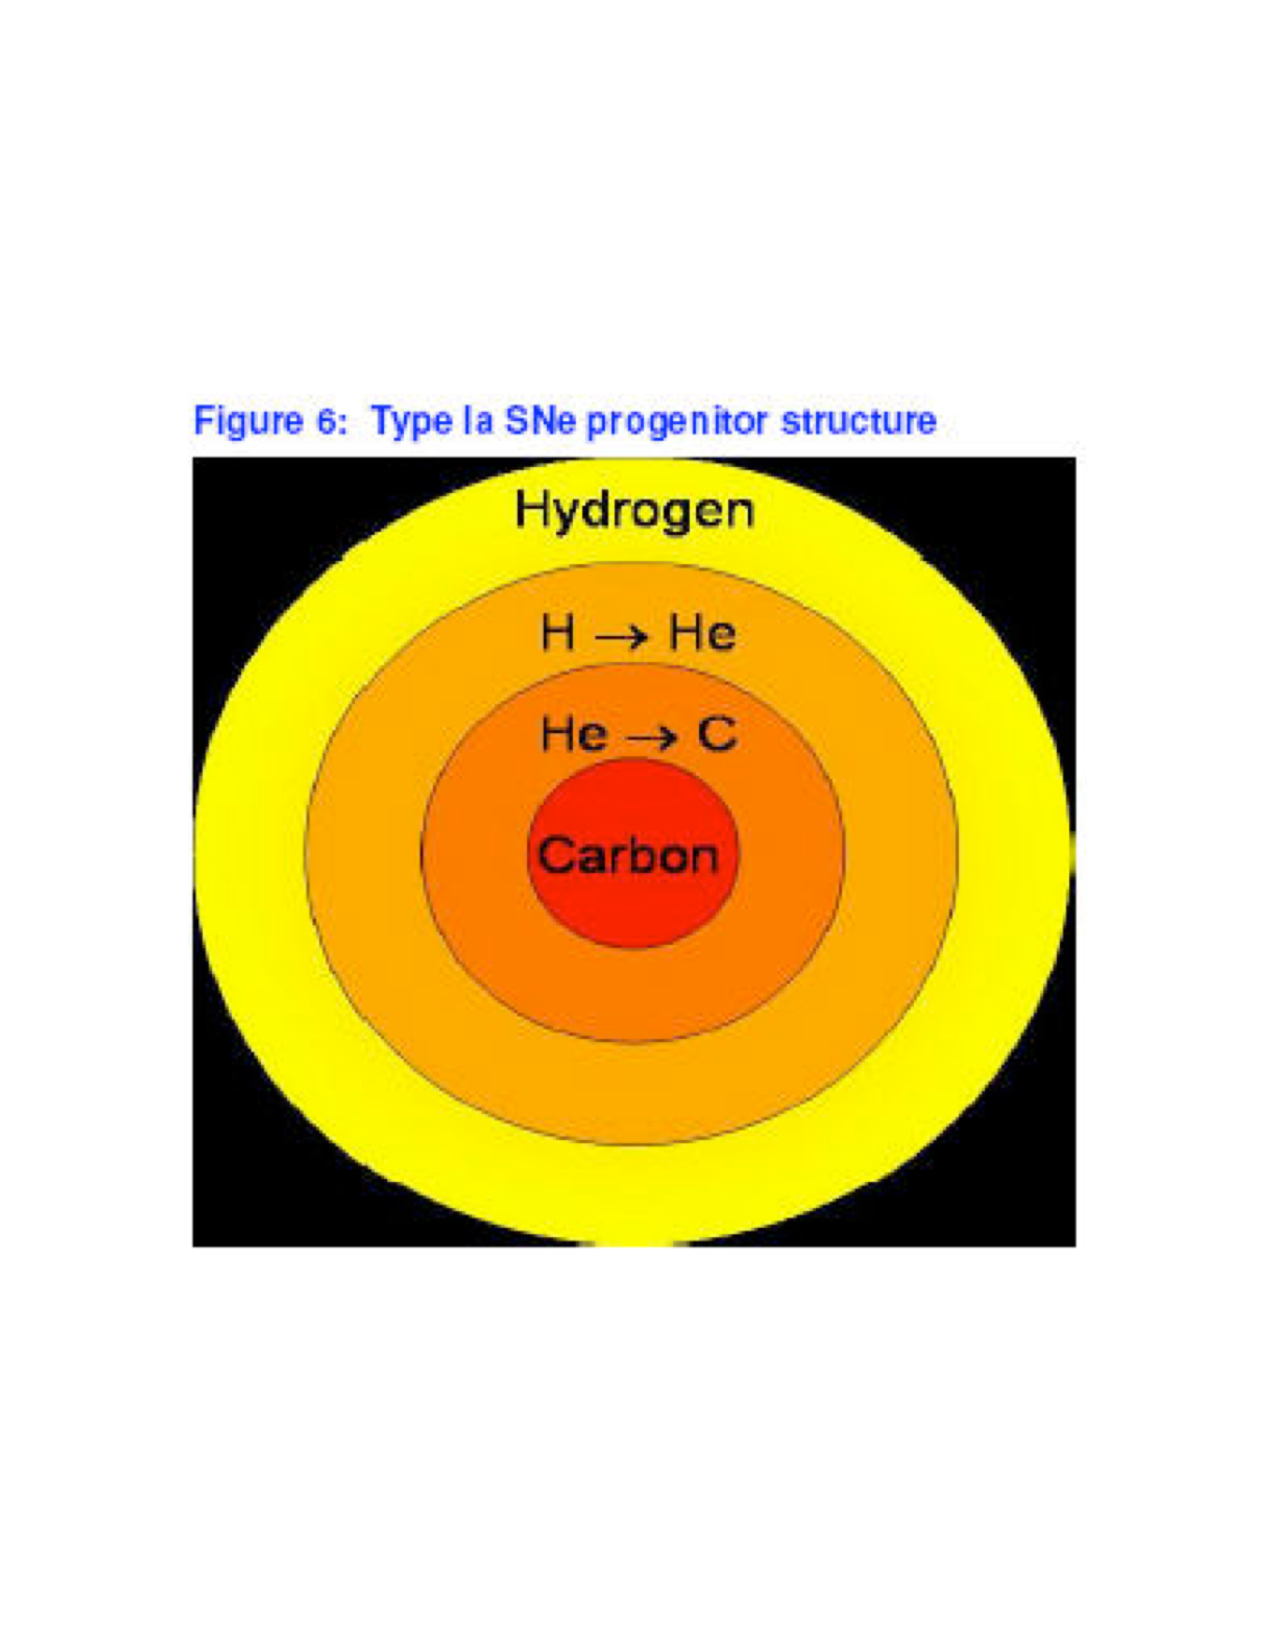
\includegraphics{figures/SN1.pdf}}
\vskip -3.6in 
\scalebox{0.7}{\hskip -1.99in 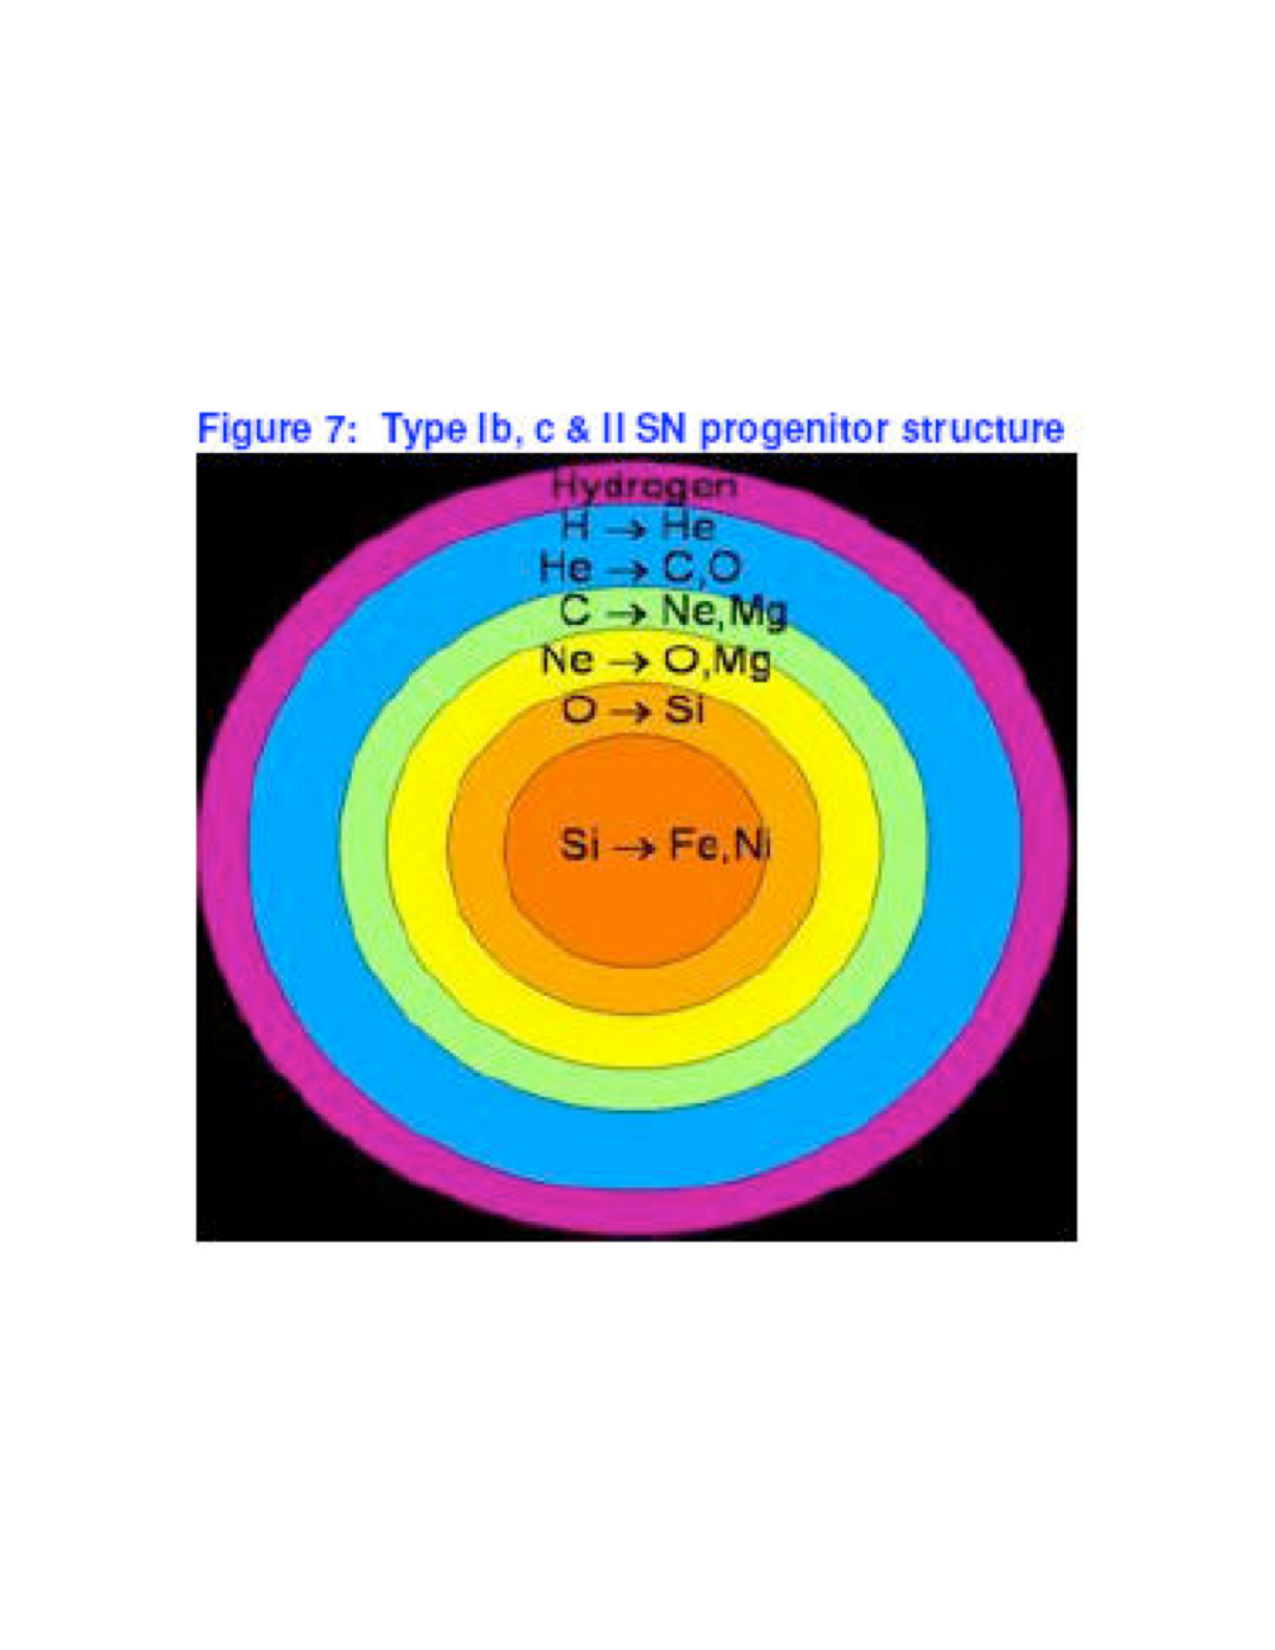
\includegraphics{figures/SN2.pdf}}
\end{center}
\end{minipage}

\begin{minipage}[t]{13cm}
\begin{center}
\vskip -1in
{\large \color{blue} Chemical yields of SNe}
\end{center}
\begin{itemize}
\item Type Ia supernovae are due to a white dwarfs in binary systems that accrete 
mass above the Chandrasekhar mass limit (1.4 $M_\odot$) and explode in a runaway 
fusion reaction (standard candles, $M_V=-19.3$, important for cosmology!). 
\item Type Ia supernovae: long time scales (of the order 1 Gyr after Type II) and net increase 
of $[Fe/H]$, while $[\alpha/Fe]$ is {\bf decreasing}! 
\item
Type II (core collapse) supernovae: short time scales and net increase 
of both $[\alpha/Fe]$ and $[Fe/H]$. 
\end{itemize}  

\end{minipage}}
\vfill 
\end{slide}

%------------------------------------------------------------------------------

%------------------------------------------------------------------------------
% TWO-SIDED PAGE 
\begin{slide}

\hbox to \hsize{
\begin{minipage}[t]{12cm}
\begin{center}
\vskip -0.3in
\scalebox{0.57}{\hskip -1.7in 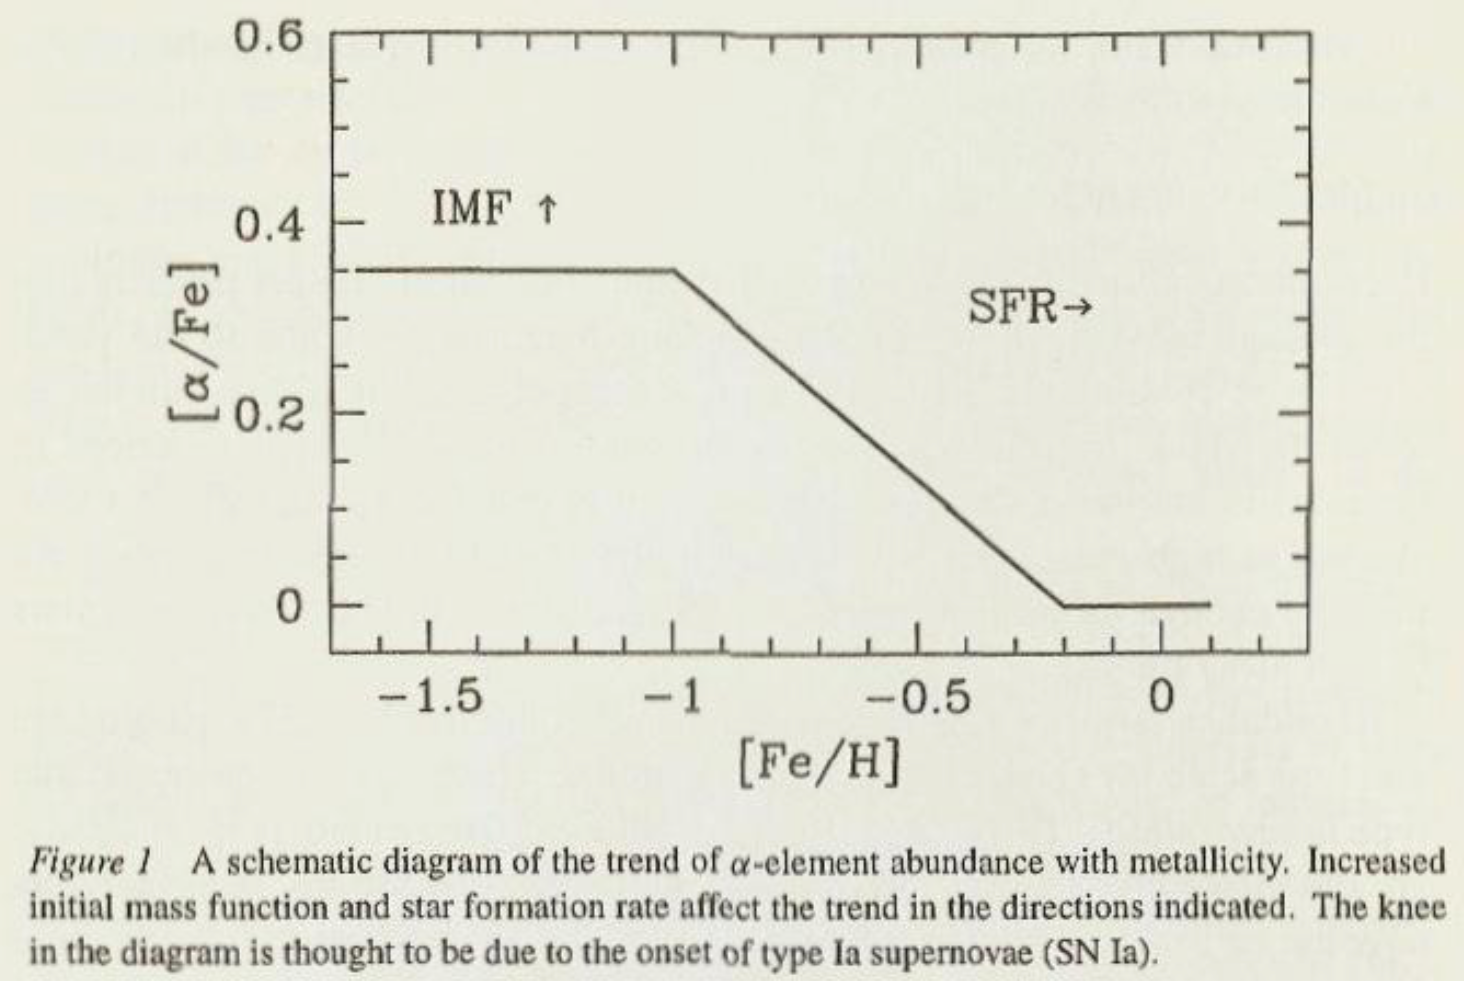
\includegraphics{figures/McWilliam.png}}
\vskip -0.05in
McWilliam \\
(1997, ARA\&A 35, 503)
\end{center}
\end{minipage}

\begin{minipage}[t]{12cm}
\begin{center}
\vskip -1in
{\large \color{red}  Generic model prediction for the path through the $[\alpha/Fe]$ vs. $[Fe/H]$ diagram}
\end{center}

\begin{itemize}
\item A population of stars starts at high $[O/Fe]$ and low  $[Fe/H]$, upper left, and
moves towards the lower right corner.
\item {\it The curve is parametrized by time, increasing from the top left towards the lower
right.}
\item Quantitative details depend on star formation rate as a function of time, SN rates and
their chemical yields, selection function, etc. 

\end{itemize}     

\end{minipage}}
\vfill 
\end{slide}
%------------------------------------------------------------------------------



%------------------------------------------------------------------------------
% TWO-SIDED PAGE 
\begin{slide}

\hbox to \hsize{
\begin{minipage}[t]{12cm}
\begin{center}
\vskip -1.1in
\scalebox{0.6}{\hskip -1.7in 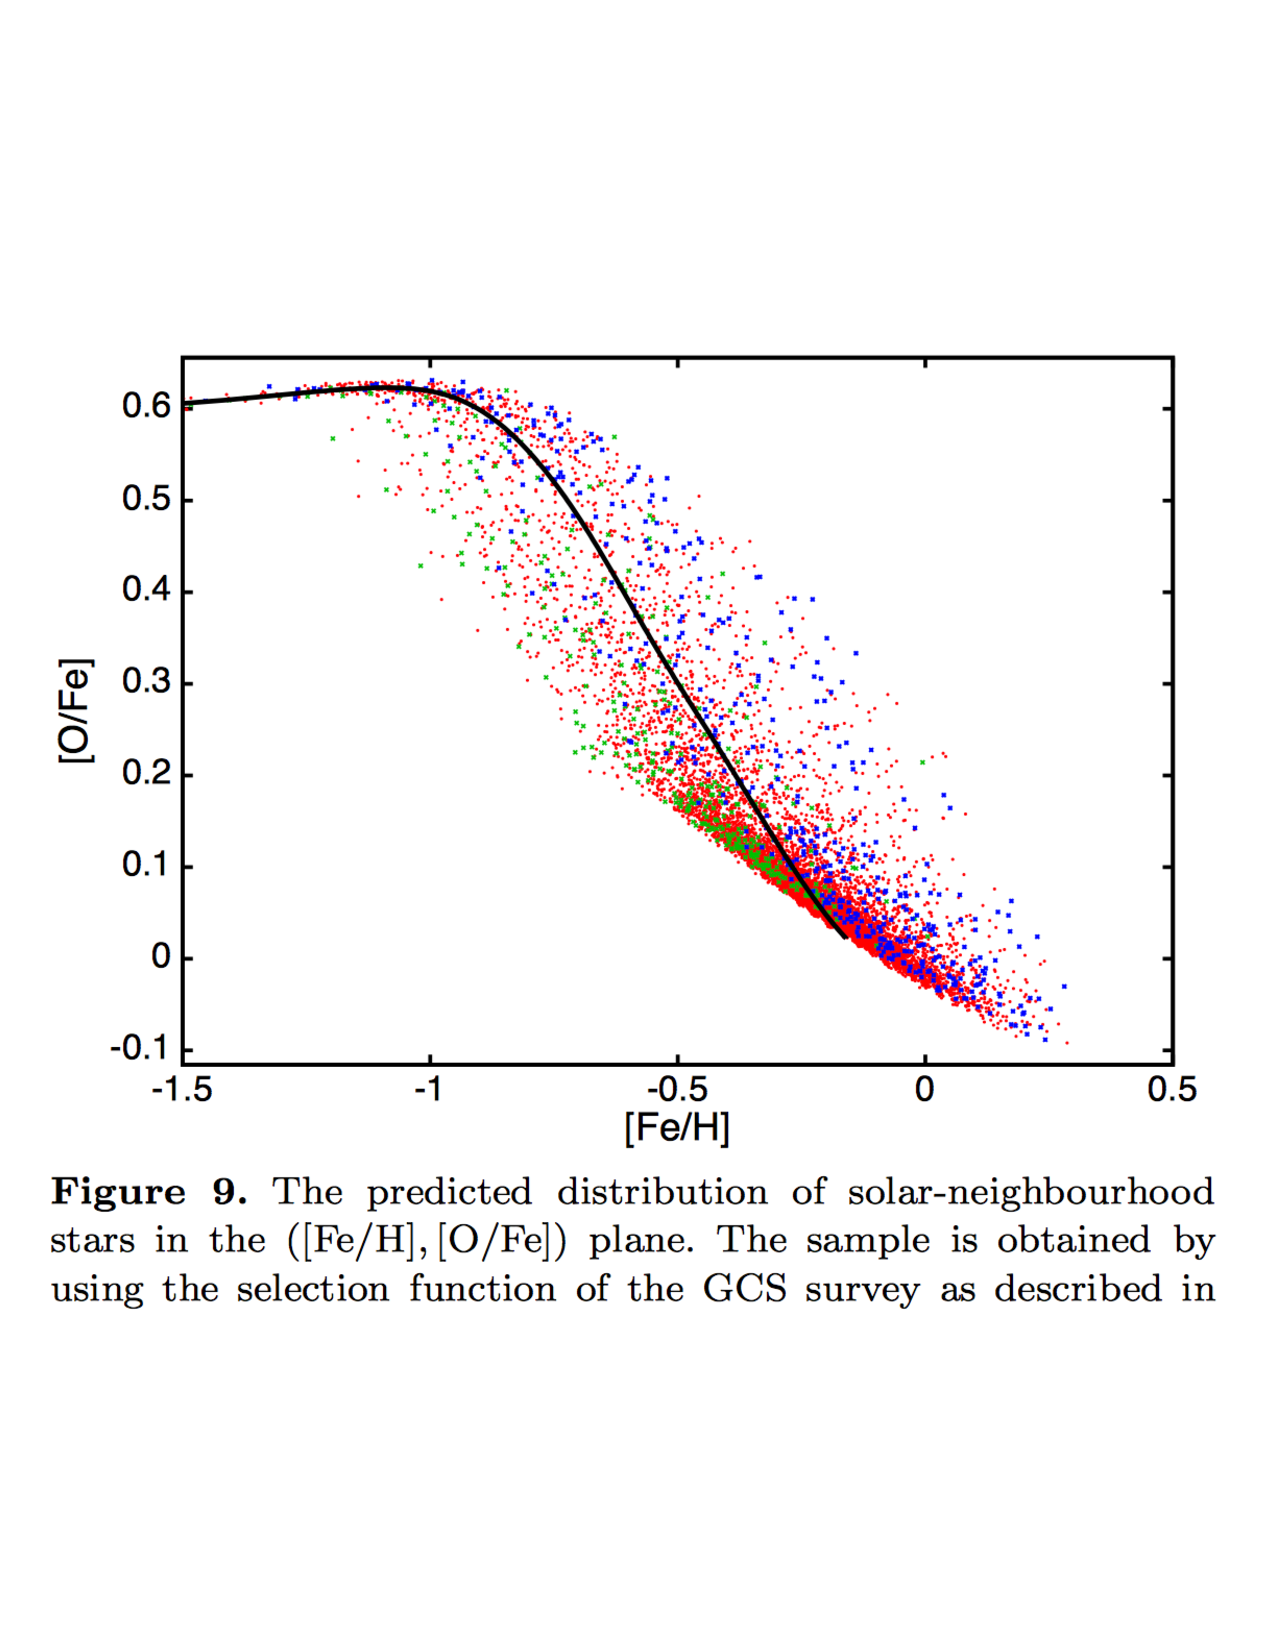
\includegraphics{figures/sb.pdf}}
\vskip -1.1in

Model-based distribution from Sch\"{o}nrich \& Binney (2009, MNRAS 396, 203). It
shows the predicted distribution of stars from the solar neighbourhood (with a selection
function from the Geneva-Copenhagen survey).

\end{center}
\end{minipage}

\begin{minipage}[t]{12cm}
\begin{center}
\vskip -1in
{\large \color{red}  Generic model prediction for the path through the $[\alpha/Fe]$ vs. $[Fe/H]$ diagram}
\end{center}

\begin{itemize}
\item A population of stars starts at high $[O/Fe]$ and low  $[Fe/H]$, upper left, and
moves towards the lower right corner.
\item {\it The curve is parametrized by time, increasing from the top left towards the lower
right.}
\item Quantitative details depend on star formation rate as a function of time, SN rates and
their chemical yields, selection function, etc. 
\item Recent progress: is the observed bimodal structure a selection effect or not? (HW 3!) 

\end{itemize}     

\end{minipage}}
\vfill 
\end{slide}
%------------------------------------------------------------------------------




%------------------------------------------------------------------------------
% TWO-SIDED PAGE 
\begin{slide}

\hbox to \hsize{
\begin{minipage}[t]{16cm}
\begin{center}
\vskip -0.6in 
\scalebox{0.9}{\hskip -1.2in 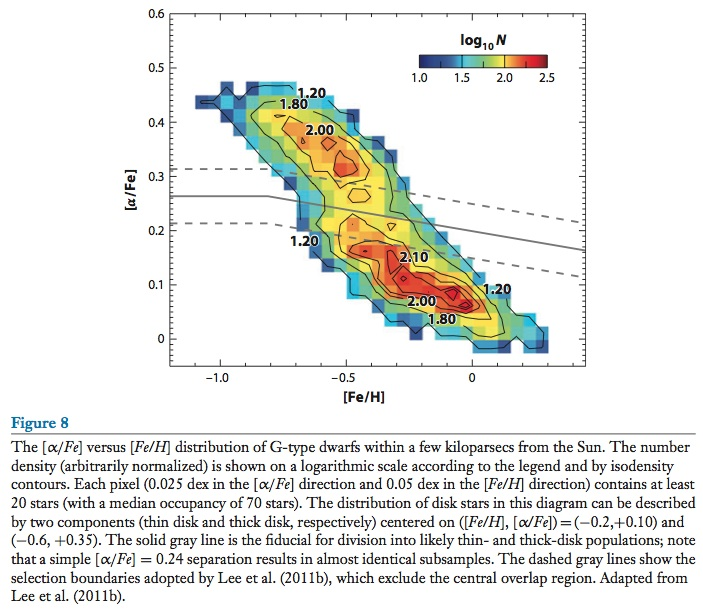
\includegraphics{figures/IBJ2012_fig8.jpg}}
\end{center}
\end{minipage}


\begin{minipage}[t]{8cm} 
\vskip -1in
\begin{center}
{\large \color{red}  $[\alpha/Fe]$ distribution for disk stars}
\end{center}
\begin{itemize}
\item 17,000 G dwarfs with  SDSS $[\alpha/Fe]$ measurements
(Lee et al. 2011).
\item {\color{blue} Bimodal distribution!} 
\item Strongly suggests a thin/thick disk separation based solely on $[\alpha/Fe]$
(age proxy?) 
\end{itemize} 
\end{minipage}}
\vfill 
\end{slide}
%-----------------------------------------------------------------------------


%------------------------------------------------------------------------------
% TWO-SIDED PAGE 
\begin{slide}

\hbox to \hsize{
\begin{minipage}[t]{12cm}
\begin{center}
\vskip -0.6in 
\scalebox{0.9}{\hskip -1.2in 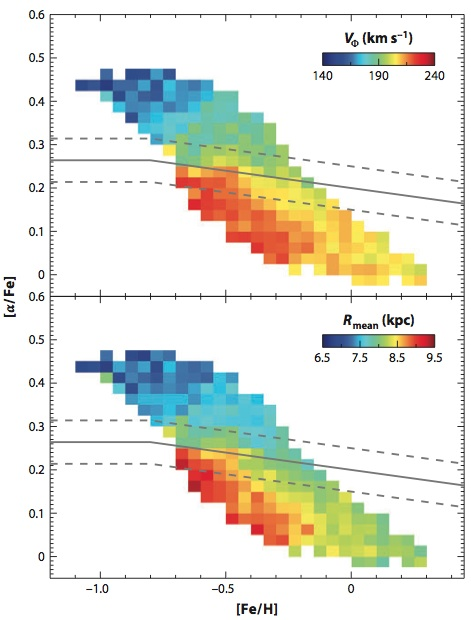
\includegraphics{figures/IBJ2012_fig9.jpg}}
\end{center}
\end{minipage}


\begin{minipage}[t]{12cm} 
\vskip -1in
\begin{center}
{\large \color{red}  $[\alpha/Fe]$ distribution for disk stars}
\end{center}
\begin{itemize}
\item Strong correlation of orbital parameters (top: rotational velocity; bottom: mean orbital radius)
with the position in the $[\alpha/Fe]$ vs. $[Fe/H]$ plane.
\item Bovy, Rix \& Hogg (2012) claim(ed) a continuous behavior rather than a two-component 
decomposition. 
\item The differences in $[\alpha/Fe]$ likely reflect {\color{blue} different star-formation timescales} 
(enrichment by Type Ia versus Type II supernovae for low and high $[\alpha/Fe]$ values over long 
and short timescales, respectively), see Bensby et al. (2004). 

\end{itemize} 
\end{minipage}}
\vfill 
\end{slide}
%-----------------------------------------------------------------------------



%------------------------------------------------------------------------------
% TWO-SIDED PAGE 
\begin{slide}

\hbox to \hsize{
\begin{minipage}[t]{12cm}
\begin{center}
\vskip -3.2in 
\scalebox{0.8}{\hskip -1.9in 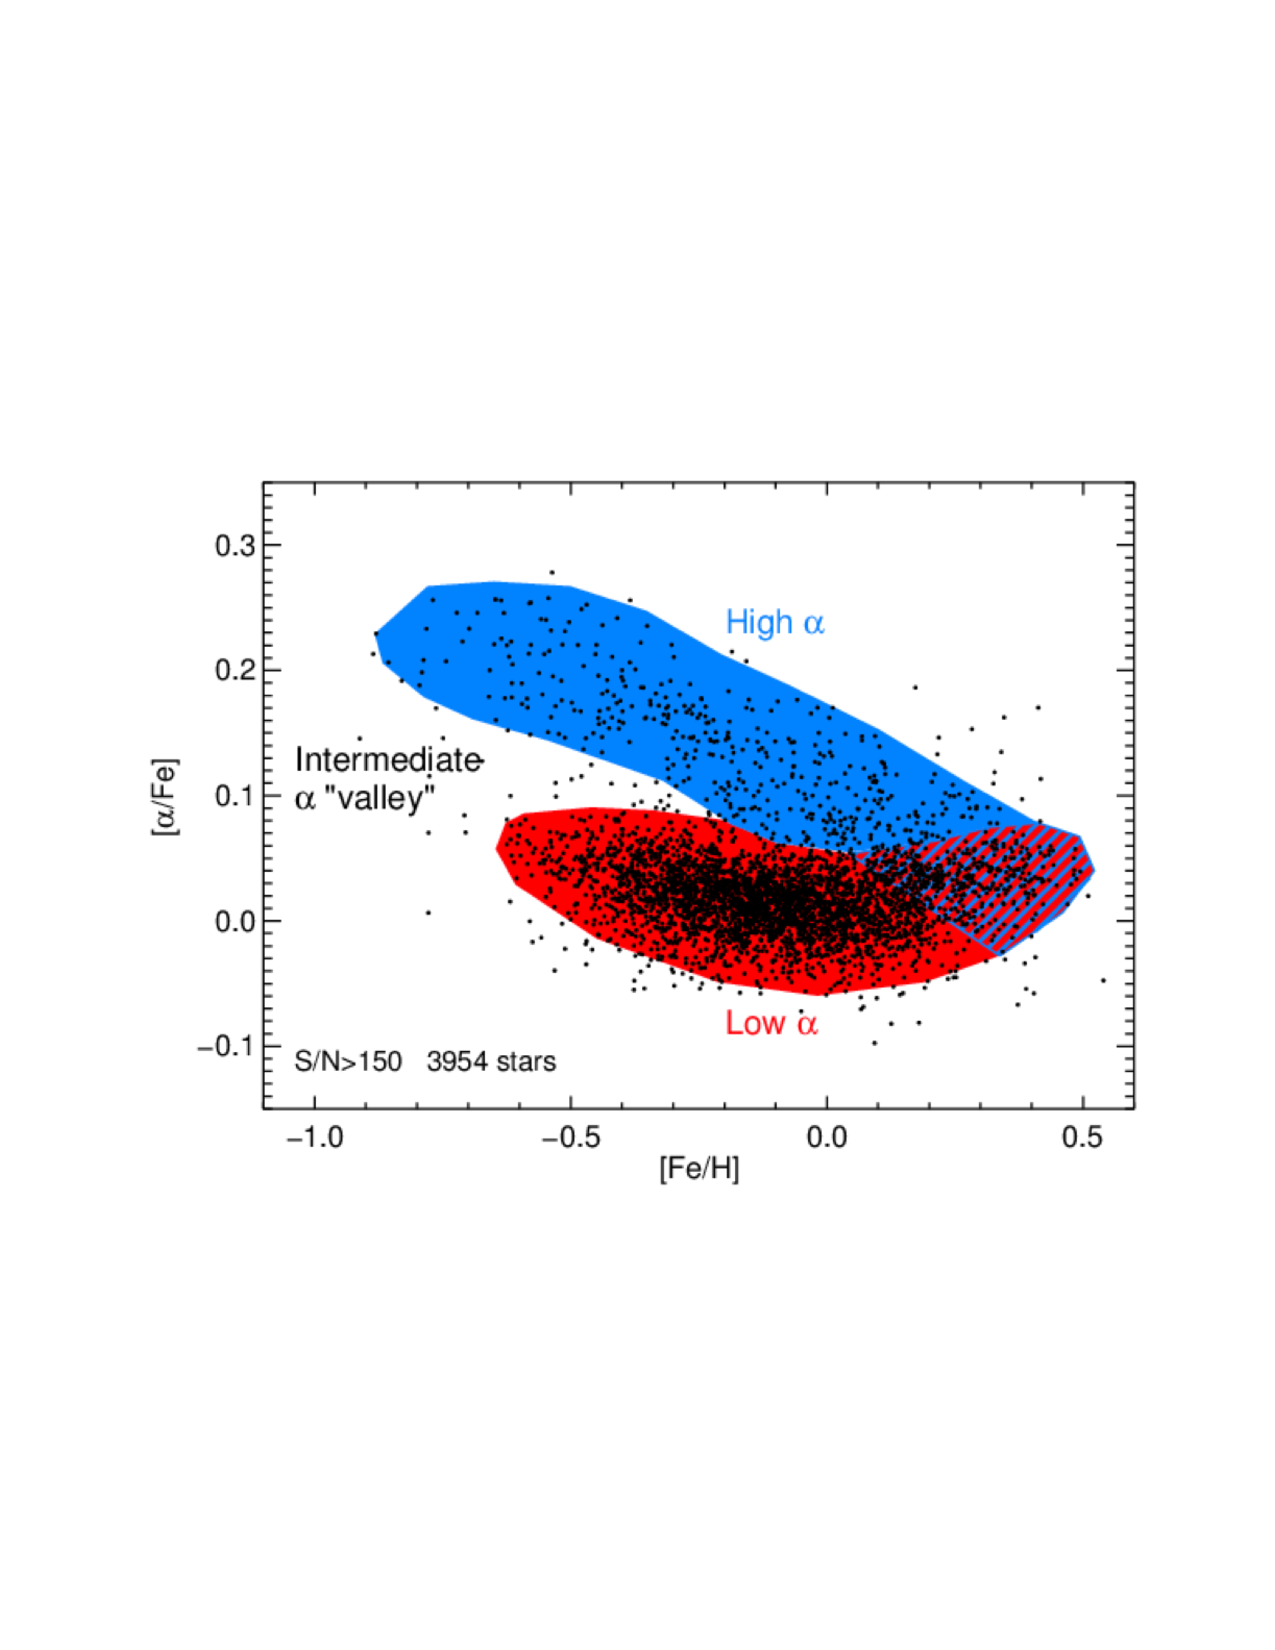
\includegraphics{figures/nidever.pdf}}
\vskip -5.1in 
\scalebox{0.9}{\hskip -2.5in 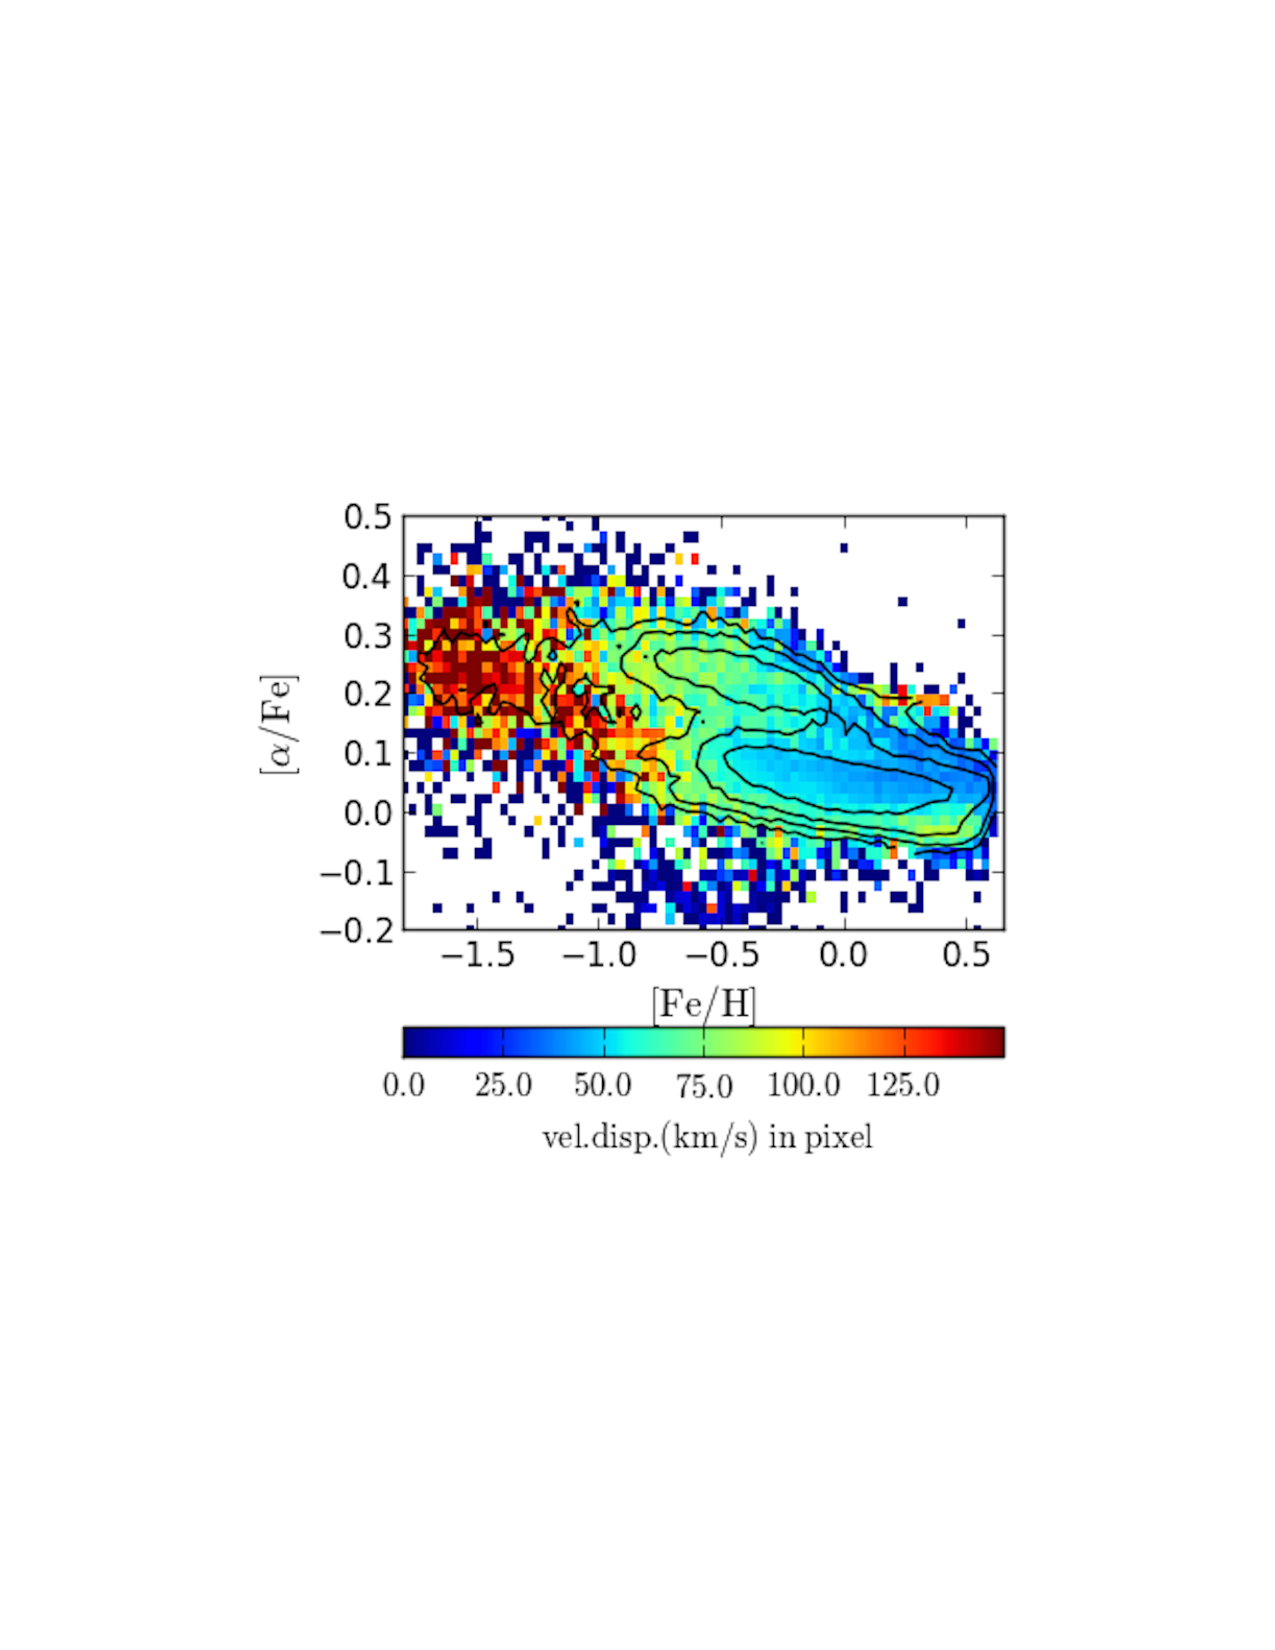
\includegraphics{figures/ziapogee.pdf}}
\end{center}
\end{minipage}


\begin{minipage}[t]{12cm} 
\vskip -1in
\begin{center}
{\large \color{red}  $[\alpha/Fe]$ distribution for disk stars}
\end{center}
\begin{itemize}
\item Latest news from Nidever, Bovy et al. (2014, ApJ 796, 38): 
``The clear $[\alpha/Fe]$ bimodality in the APOGEE data \dots
and we confirm this result \dots and find that it is not caused by selection effects.''
\item 
With APOGEE measurements (SDSS Data Release 12, bottom left), the
observed bimodality is self-evident. Also, note contamination by halo
stars at $[Fe/H] < -1$, easily recognized from elevated velocity dispersion. 
Btw, this sounds so like HW3...
\end{itemize} 
\end{minipage}}
\vfill 
\end{slide}
%-----------------------------------------------------------------------------


% 
\Spicslide{figures/HW3_figure1}{png}{}{1.0}{7}{0.0}{-0.5} 
%------------------------------------------------------------------------------




%------------------------------------------------------------------------------
% TWO-SIDED PAGE 
\begin{slide}

\hbox to \hsize{
\begin{minipage}[t]{6cm}
\begin{center}
\vskip -0.8in
\scalebox{1.0}{\hskip -0.7in 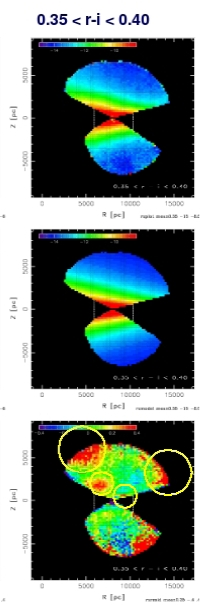
\includegraphics{figures/J08counts.jpg}}

\end{center}
\end{minipage}

\begin{minipage}[t]{17cm}
\begin{center}
\vskip -0.7in
{\large \color{red} Dissecting the Milky Way with SDSS }
\end{center}

\begin{itemize}
\item {\color{blue} Panoramic view} of the Milky Way, akin to observations 
of external galaxies; {\color{blue} good support for standard Galactic models}
(with amazing signal-to-noise!)
\item
{\color{blue} Metallicity mapping} supports components inferred 
from number counts mapping
\item
{\color{blue} Kinematics} are correlated with metallicity
\item
{\color{red} Kinematics provide constraints on gravitational potential
and initial conditions}
\end{itemize}     

\vskip 0.25in
\scalebox{0.40}{\hskip .5in 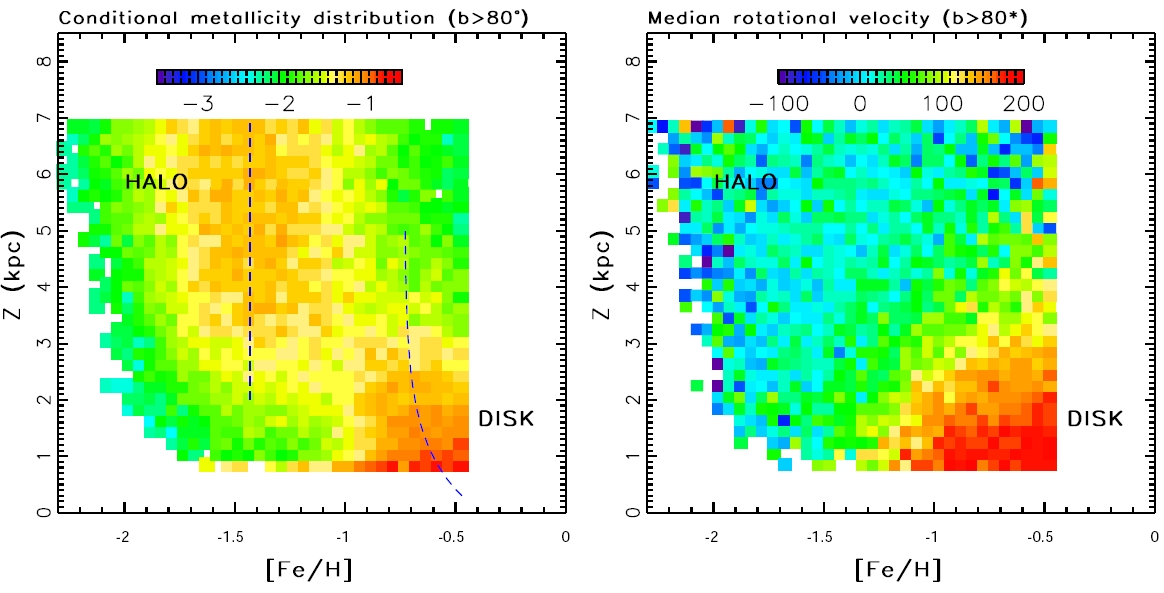
\includegraphics{figures/MetKin2panels.jpg}}

\vskip -2.5in
\scalebox{0.28}{\hskip -10.6in 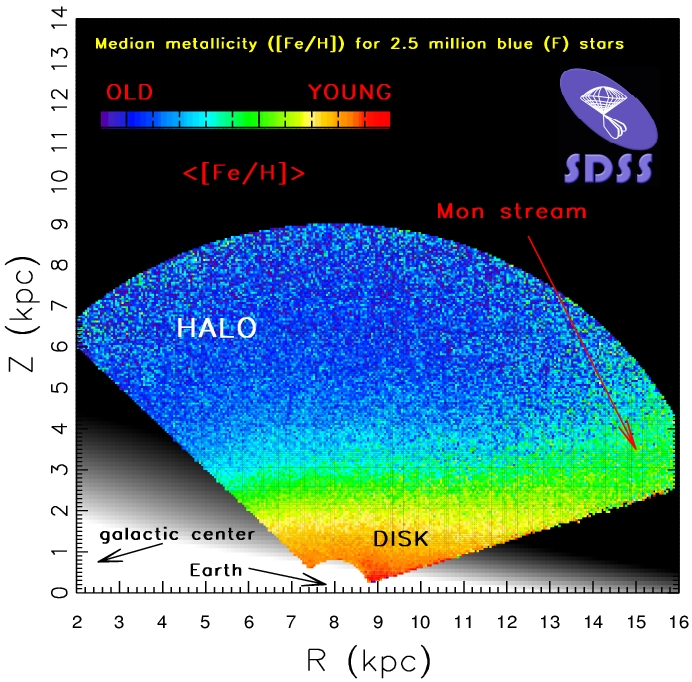
\includegraphics{figures/FeHpress.jpg}}

\end{minipage}}
\vfill 
\end{slide}
%------------------------------------------------------------------------------



%------------------------------------------------------------------------------
% TWO-SIDED PAGE 
\begin{slide}

\hbox to \hsize{
\begin{minipage}[t]{6cm}
\begin{center}
\vskip -0.8in
\scalebox{1.0}{\hskip -0.7in 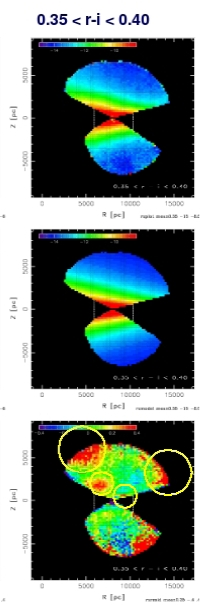
\includegraphics{figures/J08counts.jpg}}

\end{center}
\end{minipage}

\begin{minipage}[t]{17cm}
\begin{center}
\vskip -0.7in
{\large \color{red} Dissecting the Milky Way with SDSS }
\end{center}

\begin{itemize}
\item
{\bf Kinematics present a much harder analysis problem than counts
and $[Fe/H]$; instead of a single count value, or a scalar distribution
function, at each position we need to study a 3-dimensional distribution
function p($v_\Phi$, $v_R$, $v_Z$)!}
\item {\color{red} Need to measure velocities!} (Lecture 5)
\item (we can't measure acceleration -- except in special cases, such as
orbits of stars in the Galactic center as we already discussed)
\end{itemize}
     
\vskip -0.05in

\vskip 0.25in
\scalebox{0.40}{\hskip .5in 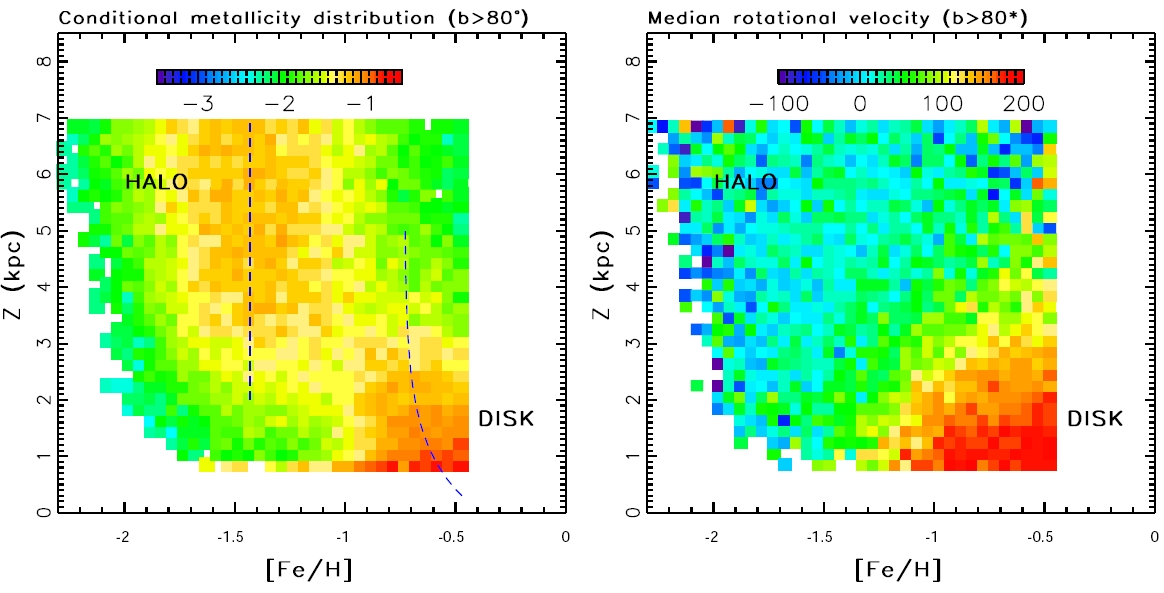
\includegraphics{figures/MetKin2panels.jpg}}

\vskip -2.5in
\scalebox{0.28}{\hskip -10.6in 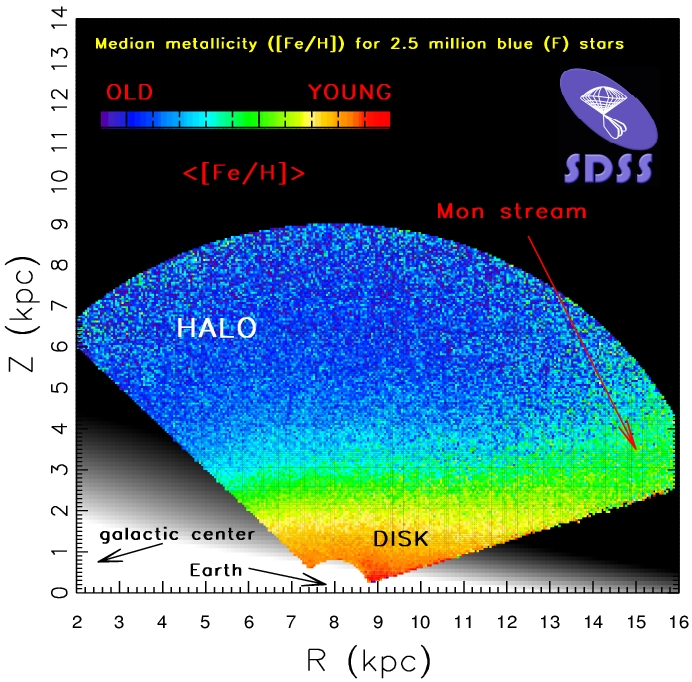
\includegraphics{figures/FeHpress.jpg}}

\end{minipage}}
\vfill 
\end{slide}
%------------------------------------------------------------------------------



%------------------------------------------------------------------------------

\begin{slide}

\begin{center}
\bfseries
\large \colour{red} Velocity measurements 
\end{center}
\vskip 0.2in
\begin{itemize}
\item Velocity can be expressed as a (vector) sum of the component 
along the line of sight, or radial velocity ($v_{rad}$), and the component
perpendicular to the line of sight, or tangential velocity ($v_{tan}$). 
\item {\color{blue} Radial velocity is measured from spectra;} large modern stellar
  spectroscopic surveys, such as SDSS and RAVE, obtain errors of a few km/s
  (a revolution: close to 10$^6$ spectra!)
\item {\color{blue} Tangential velocity is measured from proper motion:} angular displacement
   of stars on the sky (typically a tiny fraction of an arcsecond per year,
   but the record holder, Barnard's star, moves at 10 arcsec/yr);
   the two best large proper motion catalogs are based on the Hipparcos 
   survey (an astrometric satellite, accuracy of $\sim$milliarcsec/yr for $V<10$), 
   and the SDSS-POSS catalog (5$\times10^7$ stars, 3-5 mas/yr to $V<20$)
\end{itemize}    
\vfill

\end{slide}
%------------------------------------------------------------------------------


%------------------------------------------------------------------------------

\begin{slide}

\begin{center}
\bfseries
\large \colour{red} Velocity measurements 
\end{center}
\vskip 0.2in
\begin{itemize}
\item To get tangential velocity, $v$, from proper motion, $\mu$, distance $D$ 
must be known:
{\color{blue}
\begin{equation}
 v  = 4.74 \,\, {\mu \over {\rm mas/yr}} \,\, {D \over {\rm kpc} } \,\,\,\,\,\,\,\,\, {\rm km/s}
 \nonumber
\end{equation}
}
\item At a distance of 1 kpc, and for proper motions good to $\sim$mas/yr, 
the tangential velocity errors are similar to radial velocity errors from 
SDSS and RAVE
\item The advantage of radial velocity is that its measurement does not
require distance, while the advantage of proper motion measurements is
that they are much ``cheaper''
\end{itemize}    
\vfill

\end{slide}
%------------------------------------------------------------------------------




%------------------------------------------------------------------------------

\begin{slide}


\begin{center}
\vskip -2.1in
\scalebox{0.6}{\hskip -0.1in 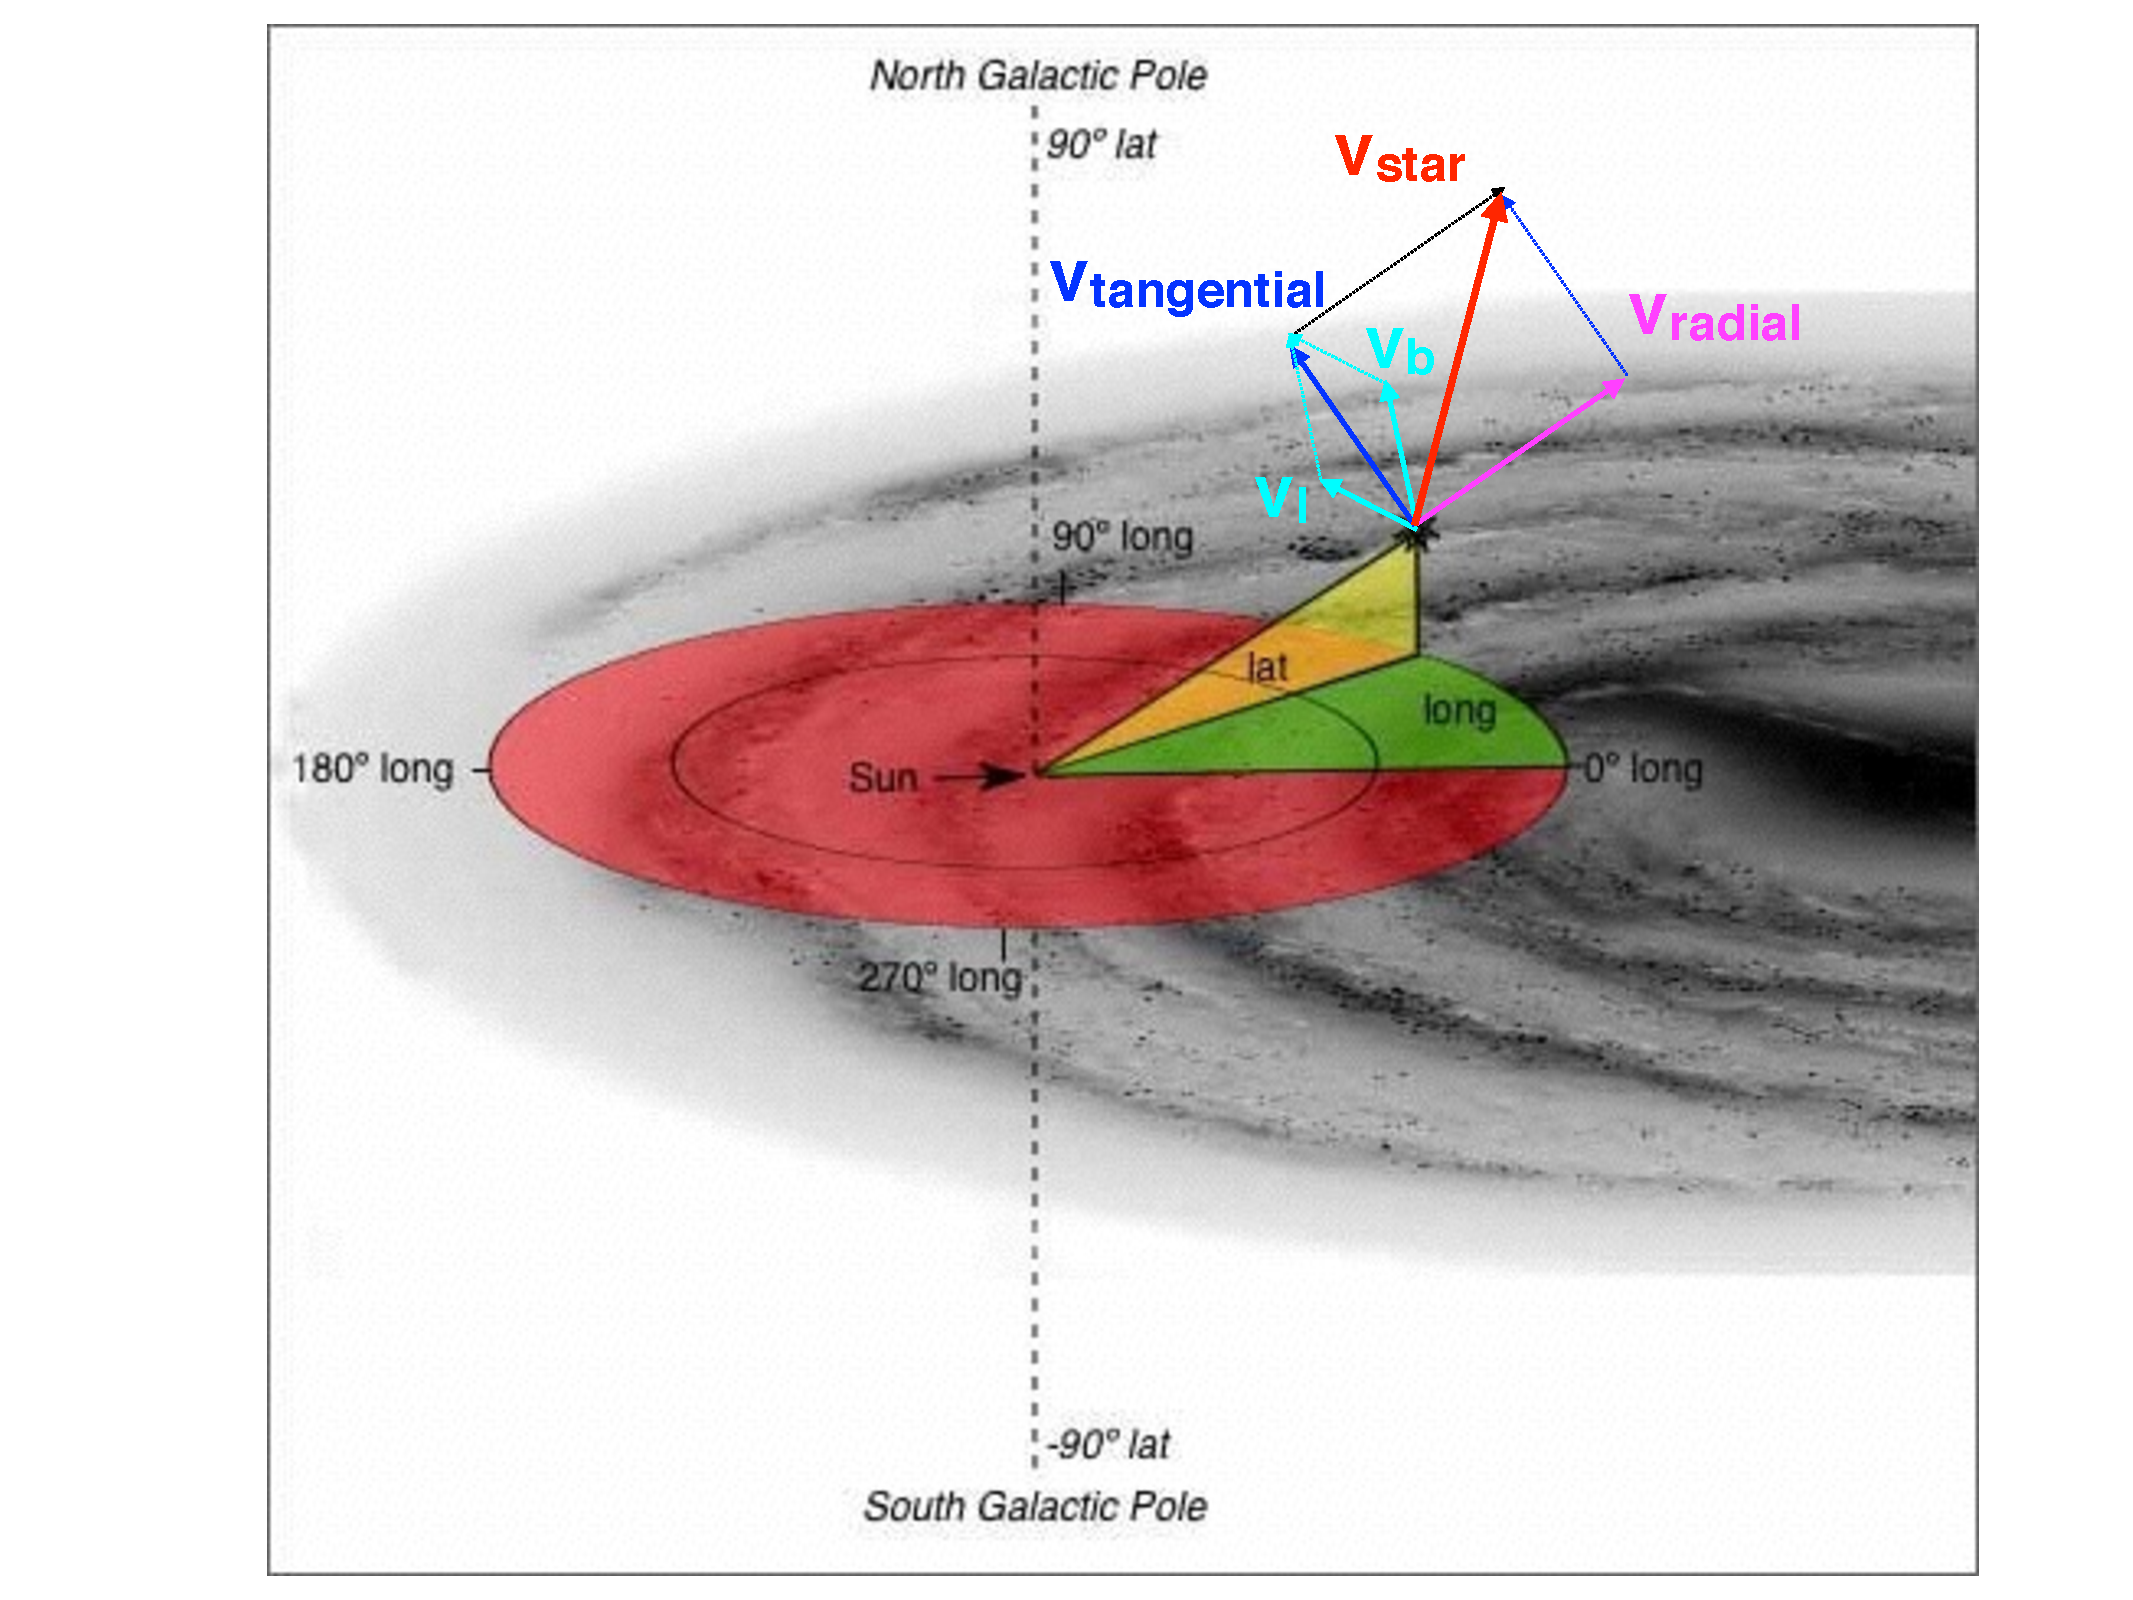
\includegraphics{figures/galacticCoordinatesAnnotatedVelocity.pdf}}
\end{center}


\vfill

\end{slide}
%------------------------------------------------------------------------------






%------------------------------------------------------------------------------

\begin{slide}

\begin{center}
\bfseries
\large \colour{red} Velocity measurements 
\end{center}
\vskip 0.2in
\begin{itemize}
\item Assume that $v_{rad}$ and the two components of tangential 
velocity, $v_l$ (in the direction of the galactic longitude) and
$v_b$ (in the direction of the galactic latitude), are known.
\item The Cartesian velocity components can be computed from 
\begin{eqnarray} 
 v_X^{obs} = -v_{rad} \cos(l) \cos(b) + v_b \cos(l) \sin(b) + v_l \sin(l) \nonumber \\
 v_Y^{obs} = -v_{rad} \sin(l) \cos(b) + v_b \sin(l) \sin(b) - v_l \cos(l) \nonumber \\
 v_Z^{obs} = -v_{rad} \sin(b) + v_b \cos(b)   \hskip 2.8in                            \nonumber
    % NB: for l=0: v_b =  vR*sin(b) + vZ*cos(b)
    %     for l=180: v_b = -vR*sin(b) + vZ*cos(b)        
\end{eqnarray} 
\item For completeness (right-handed coordinate system!): 
\begin{eqnarray} 
   X = R_\odot - D \cos(l) \cos(b)  \nonumber \\
   Y = -D \sin(l) \cos(b) \nonumber \\
   Z = D\sin(b)  \hskip 0.8in                            \nonumber
\end{eqnarray} 
\end{itemize}    
\vfill

\end{slide}
%------------------------------------------------------------------------------


%------------------------------------------------------------------------------

\begin{slide}

\begin{center}
\bfseries
\large \colour{red} Velocity measurements 
\end{center}
\vskip 0.2in
\begin{itemize}
\item Assume that $v_{rad}$ and the two components of tangential 
velocity, $v_l$ (in the direction of the galactic longitude) and
$v_b$ (in the direction of the galactic latitude), are known.
\item The Cartesian velocity components can be computed from 
\begin{eqnarray} 
 v_X^{obs} = -v_{rad} \cos(l) \cos(b) + v_b \cos(l) \sin(b) + v_l \sin(l) \nonumber \\
 v_Y^{obs} = -v_{rad} \sin(l) \cos(b) + v_b \sin(l) \sin(b) - v_l \cos(l) \nonumber \\
 v_Z^{obs} = -v_{rad} \sin(b) + v_b \cos(b)   \hskip 2.8in                            \nonumber
    % NB: for l=0: v_b =  vR*sin(b) + vZ*cos(b)
    %     for l=180: v_b = -vR*sin(b) + vZ*cos(b)        
\end{eqnarray} 
\item Locally, these components are related to more traditional nomenclature
as $v_X=-U$, $v_Y=-V$, and $v_Z=W$. 
\end{itemize}    
\vfill

\end{slide}
%------------------------------------------------------------------------------

%------------------------------------------------------------------------------

\begin{slide}

\begin{center}
\bfseries
\large \colour{red} Velocity measurements 
\end{center}
\vskip 0.2in
\begin{itemize}
\item How do we go from the measured $v_X$, $v_Y$, and $v_Z$ for
a star, to {\bf its own galactocentric} $v_R$, $v_\phi$, and $v_Z$? 
\item First, {\color{blue} we need to account for our motion}. When reporting
radial velocity, the projection of Earth's orbital motion 
(up to 30 km/s!) is typically corrected. Hence, we {\it only} 
need to correct for the solar motion around the center of the
Milky Way ($v^\odot$):
\begin{eqnarray} 
           v_X^{obs} = v_X^\ast + v_X^\odot  \nonumber \\
           v_Y^{obs} = v_Y^\ast + v_Y^\odot  \nonumber \\
           v_Z^{obs} = v_Z^\ast + v_Z^\odot  \nonumber    
\end{eqnarray} 
where $v^\ast$ corresponds to a {\bf star's own motion} around the center 
of the Milky Way (this is what we want to get)
\end{itemize}    
\vfill

\end{slide}
%------------------------------------------------------------------------------


%------------------------------------------------------------------------------

\begin{slide}

\begin{center}
\bfseries
\large \colour{red} Velocity measurements 
\end{center}
\vskip 0.2in
\begin{itemize}
\item The solar motion is traditionally decomposed into the 
{\bf rotational} motion of the Local Standard of Rest and
the solar {\bf peculiar} motion:
\begin{eqnarray} 
   v_X^\odot = v_X^{\odot,pec}             \hskip 3in   \nonumber \\
   v_Y^\odot = -v_{LSR} + v_Y^{\odot,pec }  \hskip 1.7in \nonumber \\
   v_Z^\odot = v_Z^{\odot,pec}             \hskip 3in   \nonumber       
\end{eqnarray} 
\item {\bf Note the minus sign in front of $v_{LSR}$!} Usually it is assumed
that {\color{blue} $v_{LSR}=220$ km/s} (based on HI measurements by Gunn, Knapp \& Tremaine 
1979), but some recent papers claim that it could be off by as much as 
20-30 km/s (some methods are sensitive to uncertain $R_\ast=8.0$ kpc!)
\end{itemize}    
\vfill

\end{slide}
%------------------------------------------------------------------------------


%------------------------------------------------------------------------------

\begin{slide}

\begin{center}
\bfseries
\large \colour{red} Velocity measurements 
\end{center}
\vskip 0.2in
\begin{itemize}
\item The solar peculiar motion is obtained by averaging the motions of
   a large number of stars from the (local) solar neighboorhood (so that
   their peculiar velocities cancel out)
\item Currently the best measurement of the solar peculiar motion is
   based on Hipparcos data (Dehnen \& Binney 1998): 
  {\color{blue}  $v_X^{\odot,pec}=-10.0$ km/s,  $v_Y^{\odot,pec}=-5.3$ km/s,  
   $v_Z^{\odot,pec}=7.2$ km/s.}
\item But recently they revisited this problem (Sch\"{o}nrich, Binney \& Dehnen 2010): \\
  {\color{blue}  $v_X^{\odot,pec}=-11.1$ km/s,  $v_Y^{\odot,pec}=-12.2$ km/s,  
   $v_Z^{\odot,pec}=7.3$ km/s}
\item The measured mean $Y$ velocity component depends greatly on 
   the selected type of stars (the so-called {\it asymmetric drift}).   
\end{itemize}

\vfill
\end{slide}
%------------------------------------------------------------------------------




%------------------------------------------------------------------------------

\begin{slide}

\begin{center}
\bfseries
\large \colour{red} Velocity measurements 
\end{center}
\vskip 0.2in
\begin{itemize}
\item How do we go from the measured $v_X$, $v_Y$, and $v_Z$ for
a star, to {\bf its own galactocentric} $v_R$, $v_\phi$, and $v_Z$? 
\item First, we need to account for our motion:
\begin{eqnarray} 
           v_X^\ast = v_X^{obs} - v_X^\odot  \nonumber \\
           v_Y^\ast = v_Y^{obs} - v_Y^\odot  \nonumber \\
           v_Z^\ast = v_Z^{obs} - v_Z^\odot  \nonumber   
\end{eqnarray} 
\item After ($v_X^\ast$, $v_Y^\ast$, $v_X^\ast$) are known, and assuming
that the position of the star, ($X^\ast$, $Y^\ast$, $Z^\ast$), is known 
too, this is simply a coordinate system transformation ($R=\sqrt{X^2+Y^2}$)
\begin{eqnarray} 
    v_R^\ast = v_X^\ast {X^\ast \over R^\ast} + v_Y^\ast {Y^\ast \over R^\ast}  \nonumber \\
  v_\phi^\ast = -v_X^\ast {Y^\ast \over R^\ast} + v_Y^\ast {X^\ast \over R^\ast}  \nonumber 
\end{eqnarray} 
\end{itemize}    
\vfill
\end{slide}
%------------------------------------------------------------------------------


%------------------------------------------------------------------------------
\begin{slide}
\begin{center}
\bfseries
\large \colour{red} Oort's constants 
\end{center}
\vskip 0.2in

If we have kinematic measurements for nearby stars at a range of Galactic longitudes ($l$),
\eq{
{v^{obs}_{rad}(l)\over D} = A \, \sin(2\,l)
}
\eq{
{v^{obs}_{tan}(l) \over D} = A \, \cos(2\,l) + B
}
where $D$ is star's distance and {\bf Oort's constants} $A$ and $B$ are defined as
\eq{
   A \equiv {1 \over 2} \left( {v_c \over R} - {d v_c \over dR}\right)_{R_\odot}
}
\eq{
   B \equiv - {1 \over 2} \left( {v_c \over R} + {d v_c \over dR}\right)_{R_\odot},
}
we can estimate $v_c(R_\odot)$ and the $dv_c/dR$ derivative at $R=R_\odot$. 

Note from eq. 3 that $A$ and $B$ can be estimated from proper motions only, i.e. {\bf without} radial velocities.
\vfill
\end{slide}



%------------------------------------------------------------------------------
\begin{slide}
\begin{center}
\bfseries
\large \colour{red} Oort's constants 
\end{center}
\vskip 0.2in

In the solar neighborhood,
\eq{
   A = 14.5\pm1.5 \,\, {\rm km/s/kpc}, \,\,\,\, B=-12 \pm 3 \,\, {\rm km/s/kpc}. 
}

N.B. implied proper motions for a star at 1 kpc are up to $\sim$5 mas/yr. 

Since the difference $A-B$ is not vanishing, locally the radial velocity curve is not flat.
However, note that $A-B$ is consistent with zero to within quoted uncertainties! 

For improvements to this ``epicycle'' approximation see Dehnen 1999 (AJ 118, 1190).

\vfill
\end{slide}



%------------------------------------------------------------------------------

\begin{slide}

\begin{center}
\bfseries
\large \colour{red} Velocity Distribution Function
\end{center}
\vskip 0.2in
\begin{itemize}
\item {\color{blue} Given ($v_R^\ast$, $v_\phi^\ast$, $v_Z^\ast$)
    measurements, how do we analyze them?} (hereafter, droping superscript $\ast$)
\item For a given control volume, $dV$, positioned at ($X$, $Y$, $Z$), 
and using an appropriately chosen subsample of stars described by $tags$
(e.g. $[Fe/H]$, $M_r$, mass, age), we can define a multi-dimensional distribution function,
$p(v_R, v_\phi, v_Z, X, Y, Z, tags)$, such that the 
number of stars, $dN$, in that (spatial) volume with velocities in the range
$v_i$ to $v_i+dv_i$, with $i=R,\phi,Z$, is 
\begin{eqnarray}
  dN(X,Y,Z,v_R,v_\phi,v_Z,tags) =  \hskip 2.5in \nonumber \\
    p(v_R, v_\phi, v_Z, X,Y,Z,tags) \,\, dV \, dv_R \, dv_\phi \, dv_Z     \nonumber
\end{eqnarray}
\end{itemize}    

\vfill
\end{slide}
%------------------------------------------------------------------------------


%------------------------------------------------------------------------------

\begin{slide}

\begin{center}
\bfseries
\large \colour{red} Velocity Distribution Function
\end{center}
\vskip 0.2in
\begin{itemize}
\item The normalization of this (complex!) function depends on the 
{\bf spatial variation of density profiles} which we already studied, 
metallicity distribution, 
and the {\bf luminosity function} for each Galaxy component (e.g. 
disk and halo, which in principle also depend on position). Assuming
only three tags ($M_r$, $[Fe/H]$, age), we can formally write 
($|$ means ``given'')
\begin{eqnarray}
 p({\color{blue}v_R, v_\phi, v_Z, X,Y,Z, M_r, [Fe/H], age}) = \hskip 2.5in \nonumber \\
      \phantom{x} f({\color{blue}v_R, v_\phi, v_Z } | X,Y,Z, M_r, [Fe/H], age) \hskip 1.2in \nonumber \\
      \times \rho({\color{blue}X,Y,Z }| M_r, [Fe/H], age) \hskip 2.6in \nonumber \\
      \times \Phi({\color{blue}M_r } | [Fe/H], age) 
      \times p({\color{blue}[Fe/H] } | age) 
      \times p({\color{blue} age}) \nonumber  
\end{eqnarray}
\item Here, we would like to measure and understand theoretically the {\bf shape} of
$f(v_R, v_\phi, v_Z | X,Y,Z,tags)$ (leaving normalization aside for now), and 
how it varies with ($X$, $Y$, $Z$) and as a function of various $tags$.
\end{itemize}    

\vfill
\end{slide}
%------------------------------------------------------------------------------


%------------------------------------------------------------------------------

\begin{slide}

\begin{center}
\bfseries
\large \colour{red} Velocity Distribution Function
\end{center}
\vskip 0.2in
\begin{itemize}
\item Traditionally, the measurements were confined to the solar
neighborhood (e.g. practically all Hipparcos stars are closer than
100 pc); hence, we knew little about the spatial variation of 
$f(v_R, v_\phi, v_Z | X,Y,Z,tags)$. Also, there are very few halo
stars ($<1\%$) in local samples, so the variation as a function of 
metallicity was not well measured either. 
\item Local measurements of smallish samples were consistent with
a 3-dimensional gaussian distribution: {\bf the Schwarzschild
velocity ellipsoid} 
\begin{eqnarray}
 f(v_R, v_\phi, v_Z) = \Pi_{i=1}^3 G(\bar{v_i},\sigma_i) \nonumber
\end{eqnarray}
where $\bar{v_i}$ are {\it mean velocities}, and $\sigma_i$ are
{\it velocity dispersions} in the principal directions. In a special 
case when the velocity ellipsoid is aligned with the coordinate system, 
the principal directions are the coordinate axes.

\end{itemize}    

\vfill
\end{slide}
%------------------------------------------------------------------------------



%------------------------------------------------------------------------------

\begin{slide}

\begin{center}
\bfseries
\large \colour{red} Velocity Distribution Function
\end{center}
\vskip 0.2in
{\color{blue} Within the paradigm of {\bf velocity ellipsoid}, 
some questions to ask are:}
\begin{enumerate}
\item Is this gaussian approximation supported by the data? 
      E.g. are there localized cold streams? Multiple gaussian 
      components (disk vs. halo, thin vs. thick disk)? 
\item What are the values of $\bar{v_i}$ and $\sigma_i$, and
   do they depend on position and tags such as metallicity and age? 
\item What is the orientation of the velocity ellipsoid?  
\item Can we interpret velocity ellipsoid with some ``reasonable''
      gravitational potentials?
\end{enumerate}    
{\color{blue} We will discuss here some of recent progress enabled by SDSS data (e.g., Bond et al. 2010, ApJ 716, 1)}

\vfill
\end{slide}
%------------------------------------------------------------------------------




%------------------------------------------------------------------------------
\begin{slide}
\begin{center}
\bfseries
{\color{red} \large SDSS-POSS proper motion measurements}
\end{center}
\vskip 0.1 in
\hrule

\begin{itemize}
\item
{\color{blue} The Munn et al. (2004 AJ, 127, 3034) catalog}
   \begin{itemize}
   \item recalibrated POSS astrometry using galaxies
   \item 100,000 quasars (360 per Schmidt plate) for quality 
         assessment: random errors
         3 mas/yr (per coordinate) to $r<18$, increases to 6 mas/yr 
         at $r=20$, systematic errors $\sim$0.3 mas/yr
   \item publicly available as part of SDSS Data Release 6
   \item Over 30,000,000, mostly main sequence, stars: the largest
         accurate proper motion catalog (until Gaia and LSST)
   \end{itemize}

\end{itemize}
\end{slide}


%------------------------------------------------------------------------------




%------------------------------------------------------------------------------
% TWO-SIDED PAGE 
\begin{slide}

\hbox to \hsize{
\begin{minipage}[t]{23cm}
\begin{center}
\vskip -1.2in 
{\large \color{red} Independent Test of Systematic Errors}
\begin{itemize}
\item There are lots of quasars in SDSS-POSS sample, and quasars
don't move as fast as $\sim$mas/yr. 
\end{itemize}     

\vskip 0.01in
\scalebox{0.8}{\hskip -0.1in 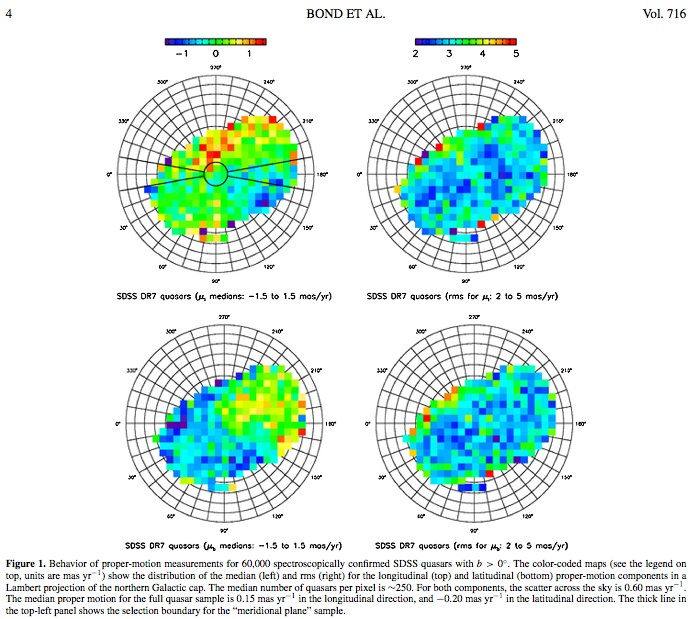
\includegraphics{figures/BondFig1.jpg}}
\end{center}
\end{minipage}

\begin{minipage}[t]{0.01cm}
\begin{center}
\vskip -0.7in 
\end{center}

\end{minipage}}
\vfill 
\end{slide}
%------------------------------------------------------------------------------




%------------------------------------------------------------------------------
% TWO-SIDED PAGE 
\begin{slide}

\hbox to \hsize{
\begin{minipage}[t]{11cm}
\begin{center}
\vskip -0.7in
\scalebox{0.7}{\hskip -1.9in 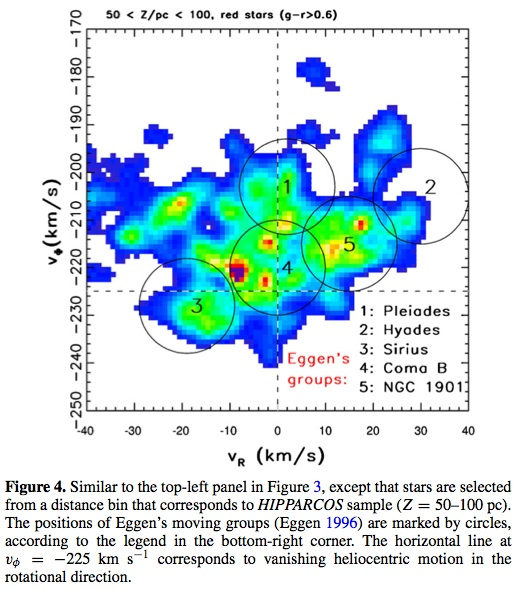
\includegraphics{figures/Bond2010_fig4.jpg}}
\vskip -0.2in
\scalebox{0.4}{\hskip -1.9in 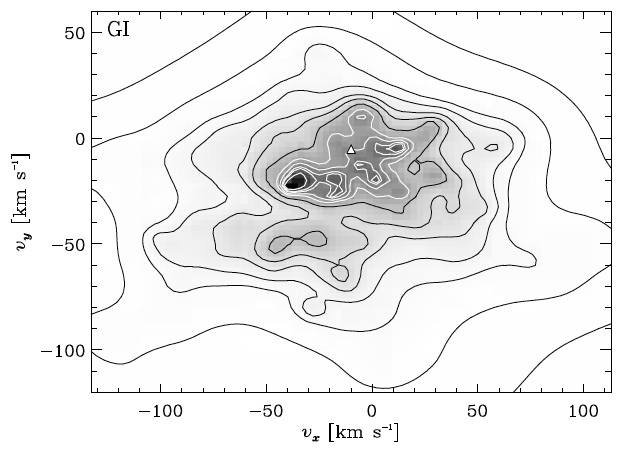
\includegraphics{figures/Dehnen1.jpg}}
\end{center}
\end{minipage}

\begin{minipage}[t]{12.5cm}
\begin{center}
\vskip -1in
{\large \color{red} Kinematics for nearby stars }
\end{center}

\begin{itemize}
\item A good summary/definitive analysis of the local Hipparcos sample: 
   Dehnen \& Binney (1998, MNRAS 298, 387).  
\item Within about 100 pc from the plane, the kinematics show a lot of
      structure: {\bf multiple peaks} (first advocated by Eggen, later
      demonstrated in Hipparcos data by Dehnen, see bottom left)
\end{itemize}     

\end{minipage}}
\vfill 
\end{slide}
%------------------------------------------------------------------------------





%------------------------------------------------------------------------------
% TWO-SIDED PAGE 
\begin{slide}

\hbox to \hsize{
\begin{minipage}[t]{8cm}
\begin{center}
\vskip -0.2in
\scalebox{0.5}{\hskip -1.4in 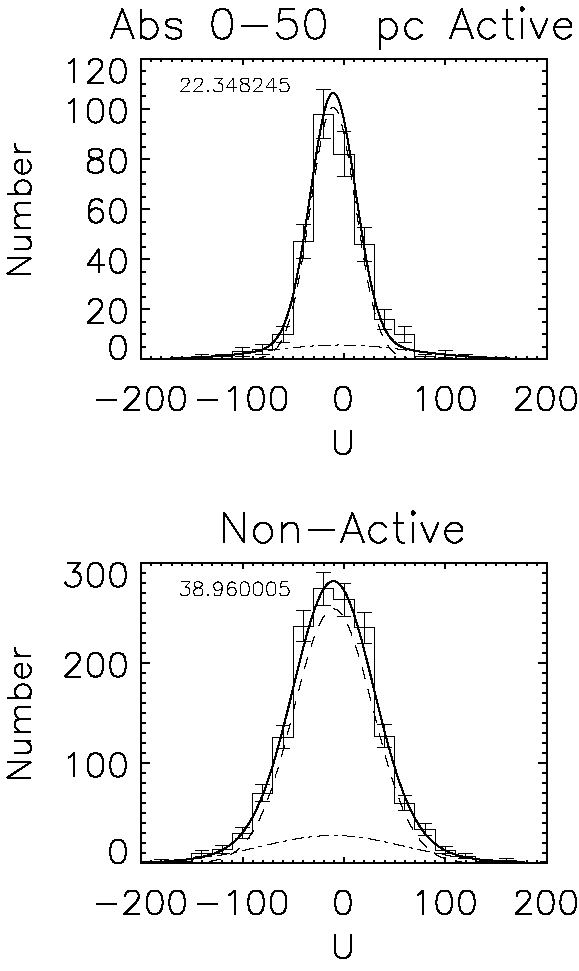
\includegraphics{figures/boo.jpg}}
Bochanski et al. (2007, AJ 134, 2418)
\end{center}
\end{minipage}

\begin{minipage}[t]{16cm}
\begin{center}
\vskip -0.9in
     {\large \color{red}  Scattering of Disk Stars  }
\end{center}

\begin{itemize}
\item Hot blue stars have smaller velocity dispersions than cool red stars;
metal-rich stars  have smaller velocity dispersions than metal-poor stars 
\item Active (presumably young) M dwarfs have smaller velocity dispersion
than non-active M dwarfs (Bochanski et al. 2007) 
\item
The imperfections in the Galaxy's gravitational field cause the random 
velocities of stars to increase: {\color{blue} the velocity dispersion increases with age:}
{\color{red} $\sigma \propto t^{1/2}$}
\item The irregularities responsible for this phenomenon range in scale 
from small such as {\color{blue} molecular clouds}, to large such as {\color{blue} 
spiral arms}
\item
Can we (at least qualitatively) understand this behavior?
\end{itemize}     

\end{minipage}}

\vfill 
\end{slide}
%------------------------------------------------------------------------------





%------------------------------------------------------------------------------
\begin{slide}

{\color{blue} \bf Scattering by molecular clouds} 

Typical clouds: up to 10$^6$ M$_\odot$, $<$100 pc

Spitzer \& Schwarzschild (1953) proposed their existence,
motivated by the correlation between the velocity dispersion
and age, {\it before} the first ones were detected!

A star has a relative speed with respect to a cloud because of
differential rotation. The successive encounters will 
increase the star's random velocity.

{\color{blue} Prediction: $\sigma \propto t^{1/4}$} 
{\color{red} slower than observed}

Another difficulty: can explain $\sigma$ of up to 30 km/s,
but white dwarfs and C stars have $\sigma \sim 50$ km/s



\vfill
\end{slide}

%------------------------------------------------------------------------------


%------------------------------------------------------------------------------
\begin{slide}

{\color{blue} \bf Scattering by spiral arms} 

N-body simulations: spiral arms can heat the disk

The spiral structure heats the disk, which decreases the 
efficiency of the swing amplifier until the spiral structure
cannot be maintained. 

{\color{blue} ``Thus the spiral structure is killed by the 
heat that it injects into the disk, just as yeast in a vat of
fermenting beer is killed by the alcohol it creates'' (from Binney
\& Tremaine).} 

Important: a fixed spiral pattern cannot heat the disk -- the
arms must be transitory (see BT figs. 7-26 and 7-27)

Note that within Lin-Shu theory disk heating is negligible;
the stochastic theory predicts significant disk heating

{\color{blue} Prediction: $\sigma \propto t^{\alpha}$, with
$\alpha\sim0.2-0.5$} not too bad



\vfill
\end{slide}

%------------------------------------------------------------------------------




%------------------------------------------------------------------------------
\begin{slide}

{\color{blue} \bf Scattering by spiral arms} 

Problem: the velocity dispersion increases only in the
radial and azimuthal directions. What about the vertical
dispersion? 

Carlberg (1984): spiral arms provide heating in the radial and azimuthal 
directions, which molecular clouds redistribute in the vertical direction.

Lacey \& Ostriker (1985): the heating is due to 10$^6$ M$_\odot$ 
black holes from the halo.



\vfill
\end{slide}

%------------------------------------------------------------------------------









%------------------------------------------------------------------------------
% TWO-SIDED PAGE 
\begin{slide}

\hbox to \hsize{
\begin{minipage}[t]{11cm}
\begin{center}
\vskip -1.0in
\scalebox{0.7}{\hskip -1.9in 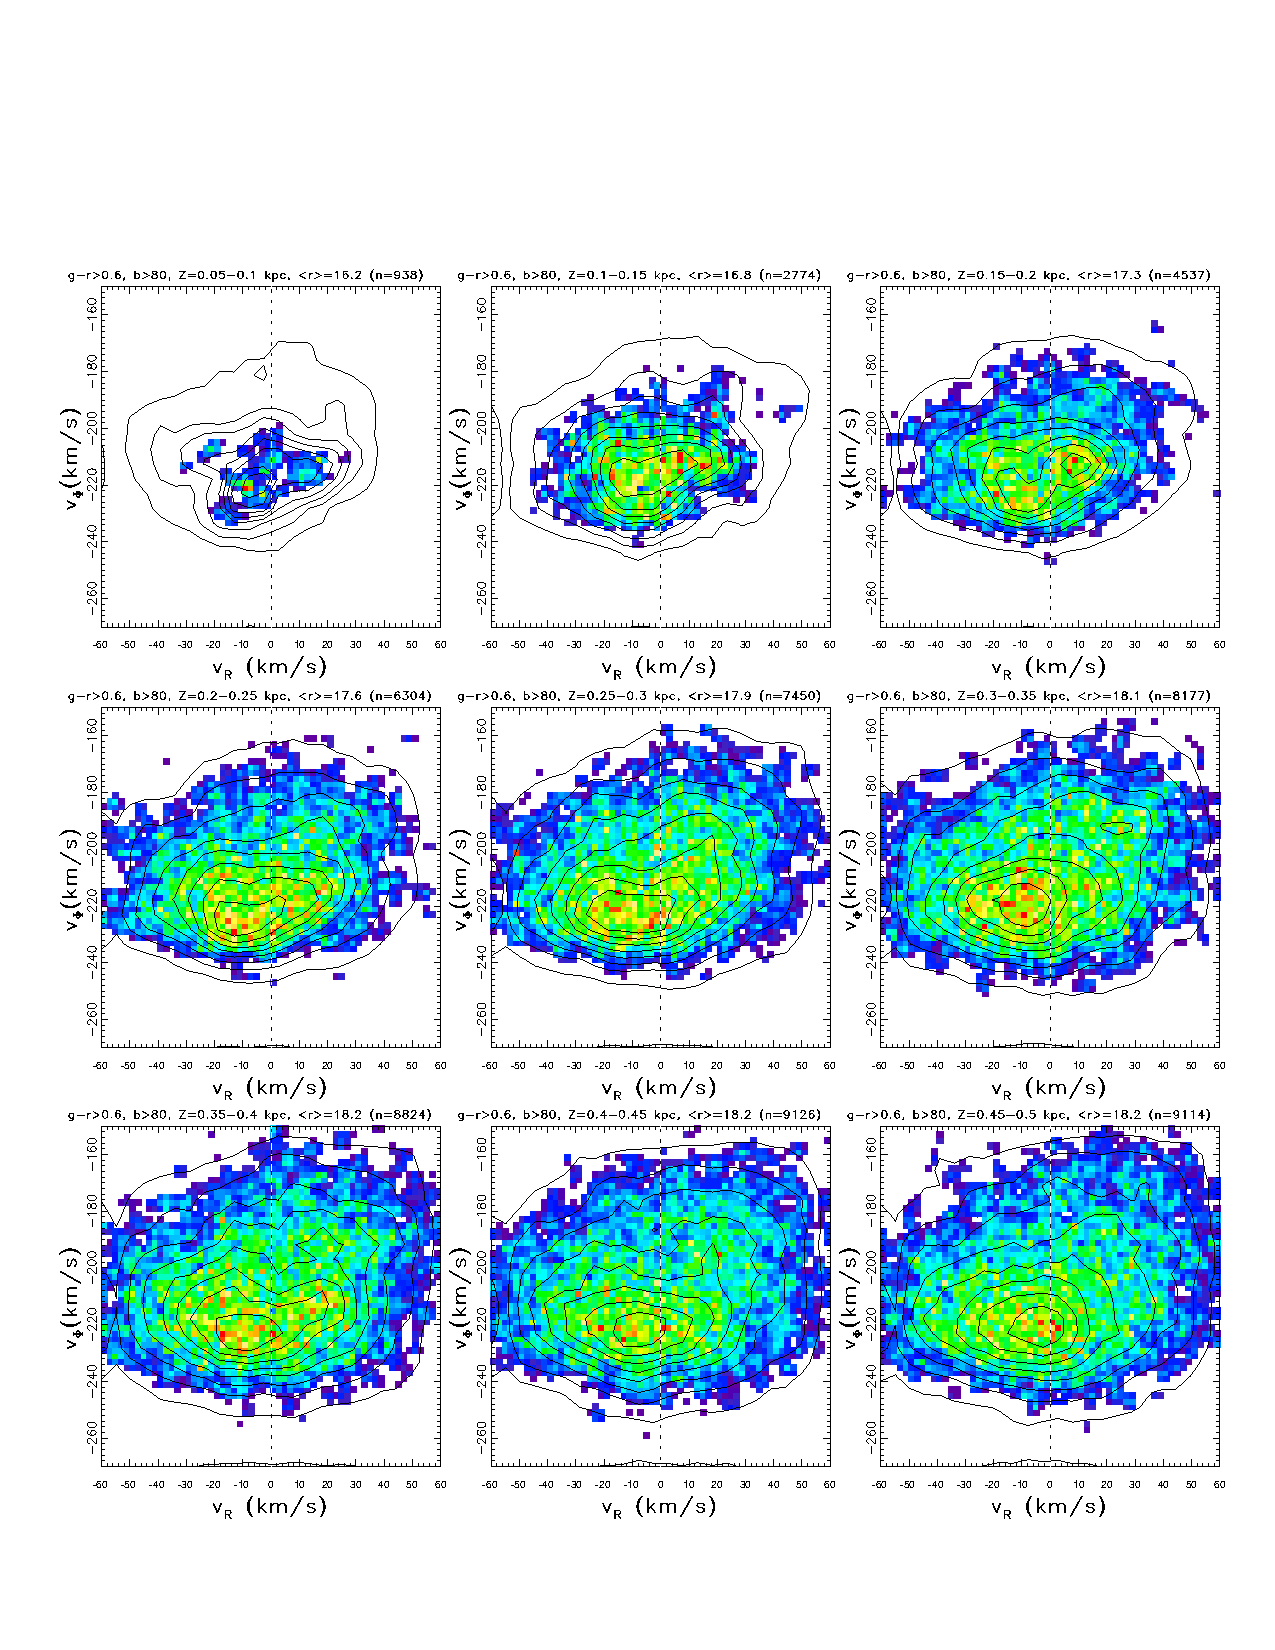
\includegraphics{figures/panelsVVmaps2_NGP_Zslices_R2.pdf}}
\end{center}
\end{minipage}

\begin{minipage}[t]{12.5cm}
\begin{center}
\vskip -1in
{\large \color{red} Kinematics for nearby stars }
\end{center}

\begin{itemize}
\item Within about 100 pc from the plane, the kinematics show a lot of
      structure: {\bf multiple peaks} (first advocated by Eggen, later
      demonstrated in Hipparcos data by Dehnen)
\item {\bf Panels:} $f(v_R, v_\phi)$ for red (K and M) main-sequence
      stars towards the north galactic pole; determined using SDSS-POSS
      proper motions, in nine 50pc thick $Z$ slices, from 50 pc to 500
      pc
\item Beyond 100 pc from the plane, the velocity distribution becomes
      more similar to a gaussian; however, deviations are clearly 
      detected (due to a large number of stars and well-controlled errors)
\end{itemize}     

\end{minipage}}
\vfill 
\end{slide}
%------------------------------------------------------------------------------




%------------------------------------------------------------------------------
% TWO-SIDED PAGE 
\begin{slide}

\hbox to \hsize{
\begin{minipage}[t]{11cm}
\begin{center}
\vskip -4.0in
\scalebox{0.7}{\hskip -1.9in 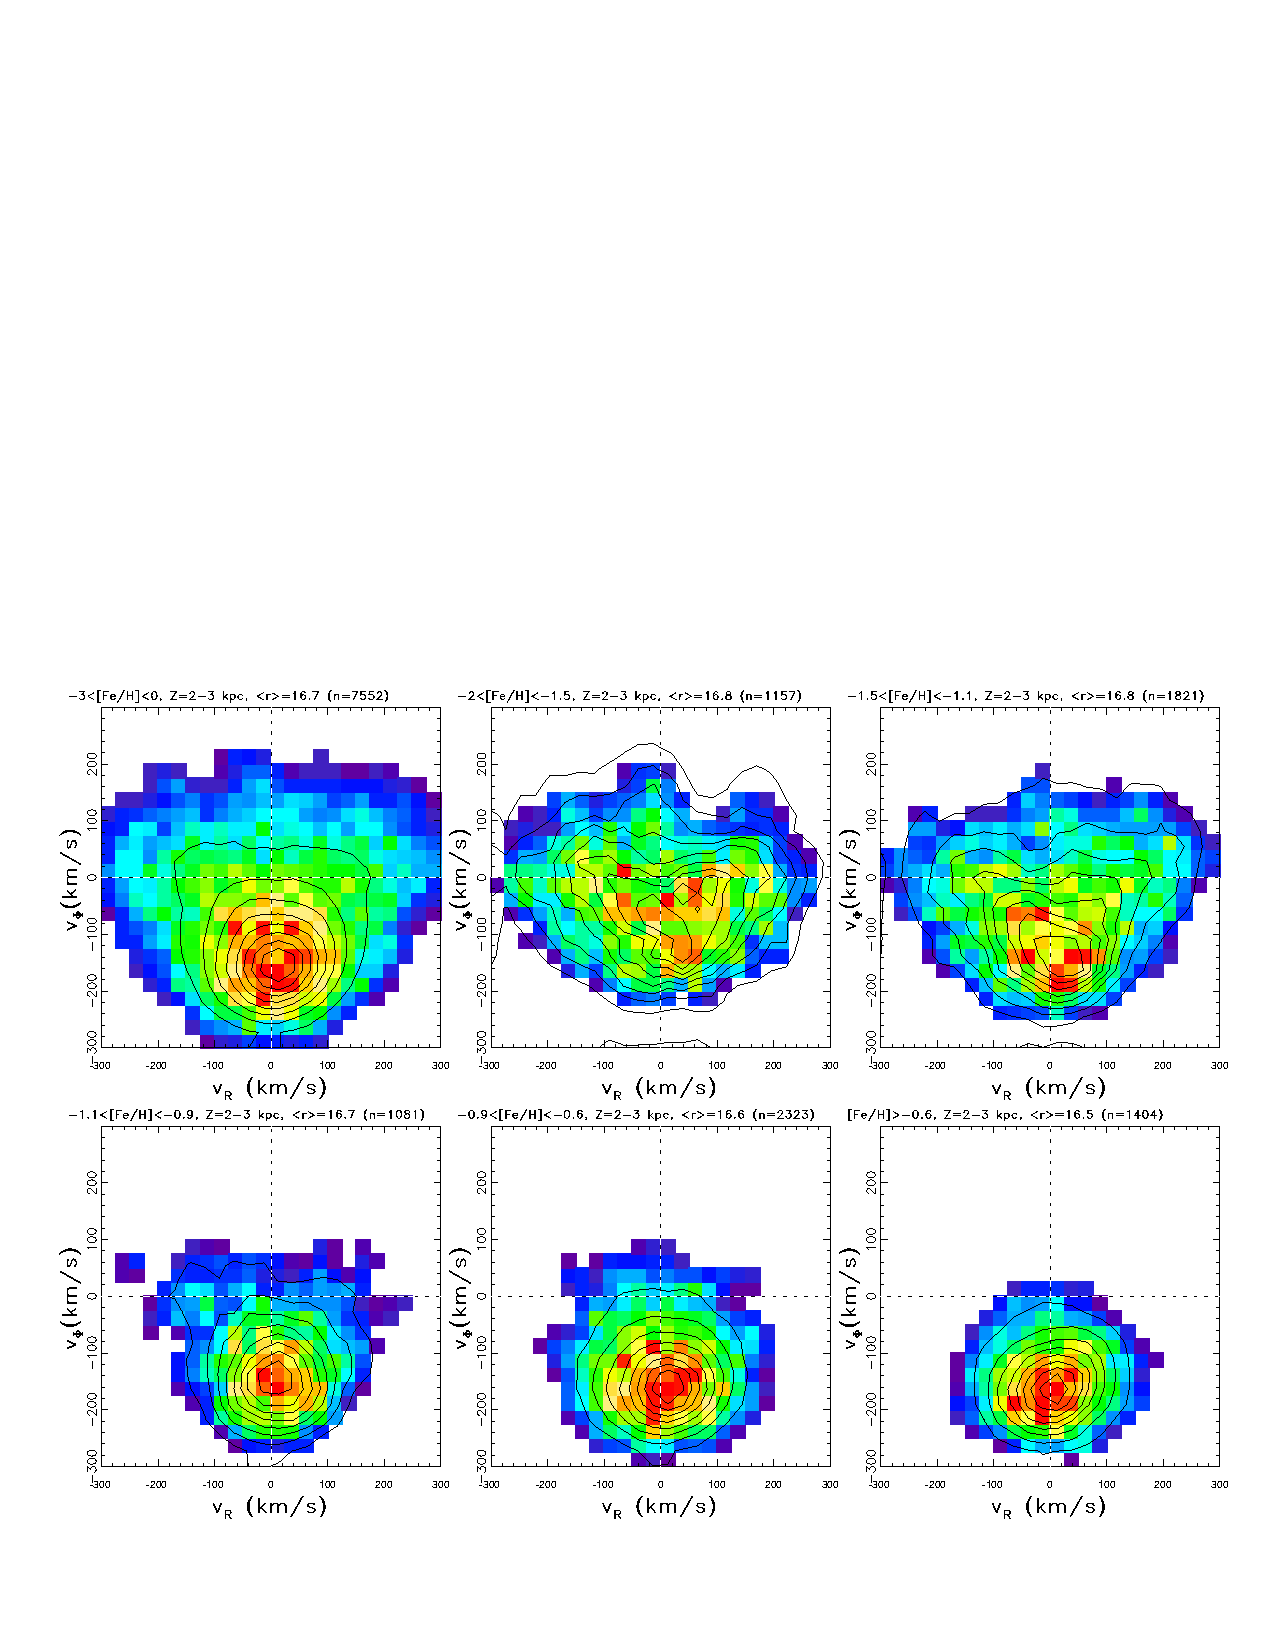
\includegraphics{figures/panelsVVmaps2_NGP_Zslices_FG2.pdf}}
\vskip -3.2in
\scalebox{0.7}{\hskip -1.9in 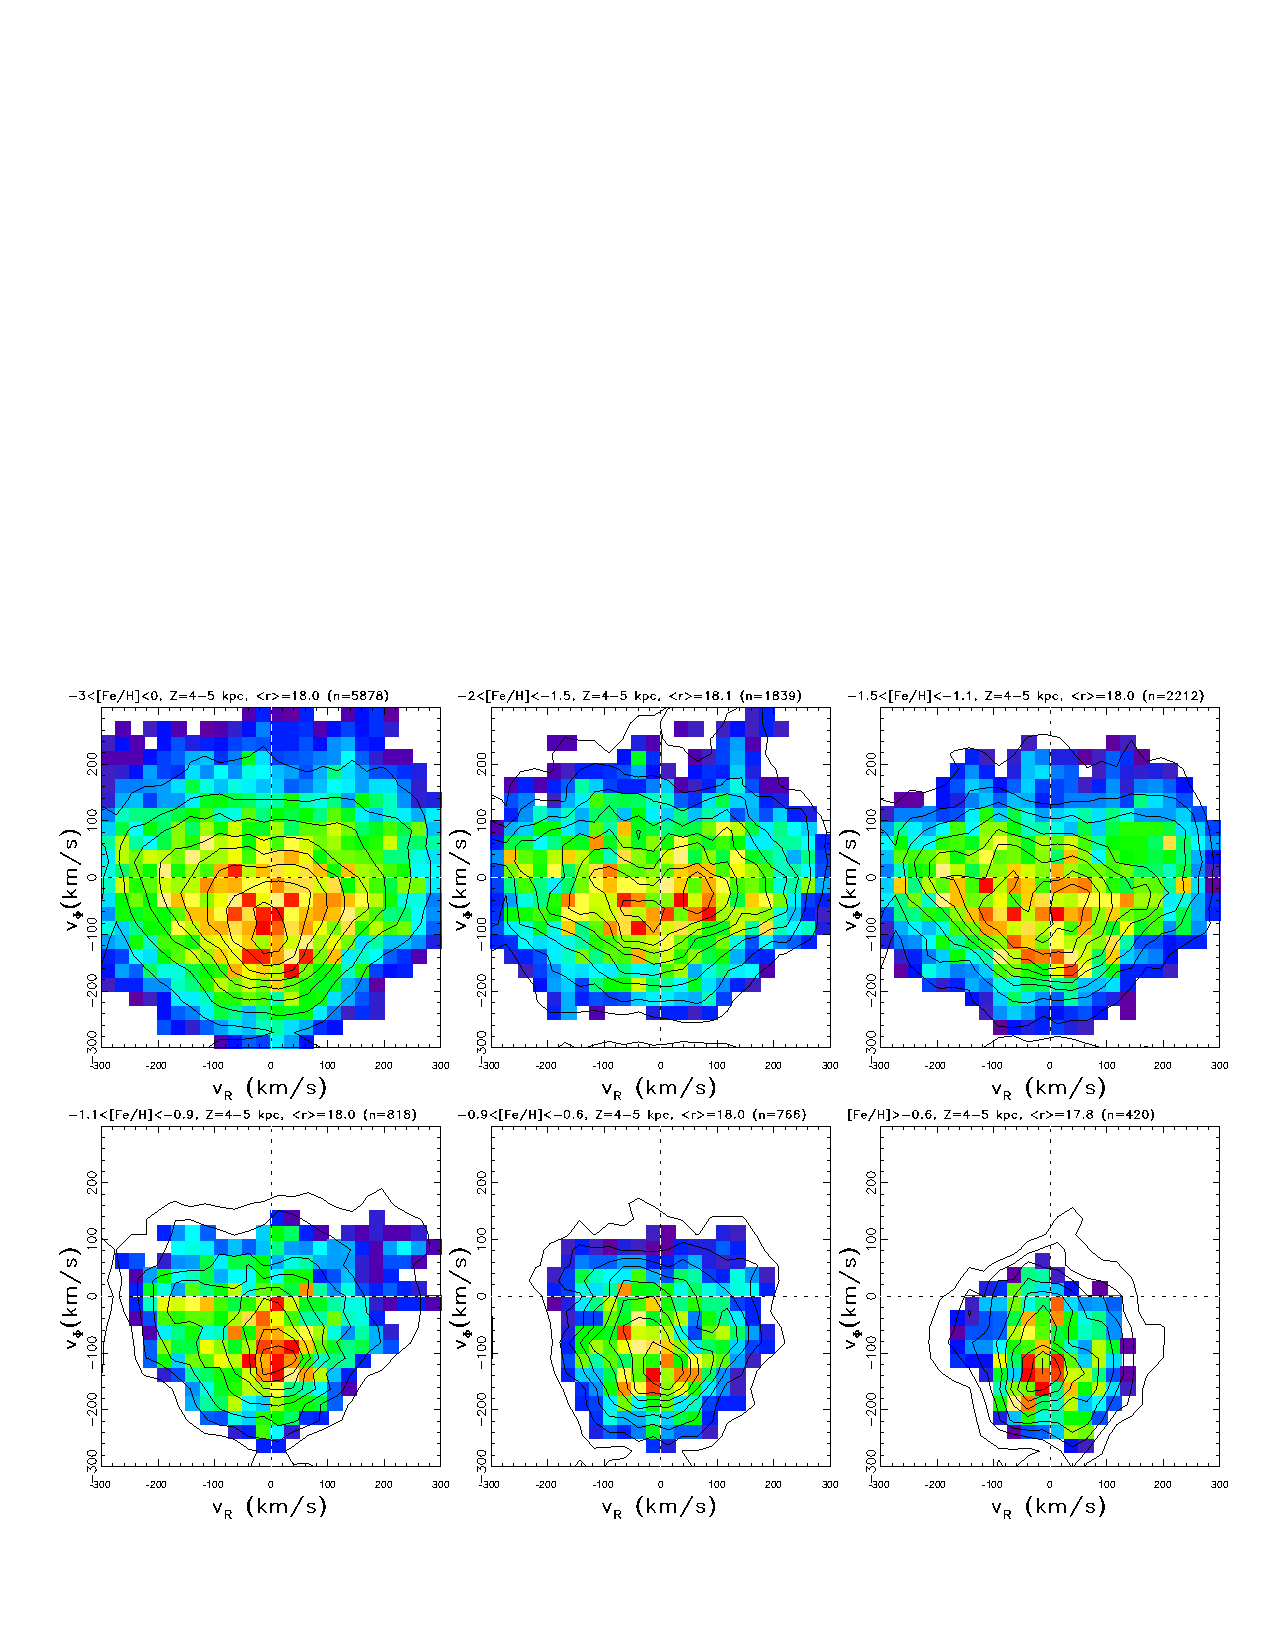
\includegraphics{figures/panelsVVmaps2_NGP_Zslices_FG4.pdf}}
\end{center}
\end{minipage}

\begin{minipage}[t]{12.5cm}
\begin{center}
\vskip -1in
{\large \color{red} Kinematics for distant stars }
\end{center}

\begin{itemize}
\item {\bf Top panels:} $f(v_R, v_\phi)$ for blue (F and G) main-sequence
      stars towards the north galactic pole; determined using SDSS-POSS
      proper motions, $Z=2-3$ kpc. The top left is the full sample, 
      the other five are for $[Fe/H]$ slices, from $-2$ to $> -0.6$
      (halo, halo, mixed, disk, disk)
\item {\bf Bottom panels:} analogous, for $Z=4-5$ kpc.
\item {\color{blue} {\bf Conclusion:} High-metallicity stars have net
      rotation (the median velocity depends on $Z$), low-metallicity
      stars are consistent with no rotation. }
\end{itemize}     

\end{minipage}}
\vfill 
\end{slide}
%------------------------------------------------------------------------------

 
 

%------------------------------------------------------------------------------
% TWO-SIDED PAGE 
\begin{slide}

\hbox to \hsize{
\begin{minipage}[t]{12cm}
\begin{center}
\vskip -0.5in
\scalebox{0.7}{\hskip -1.6in 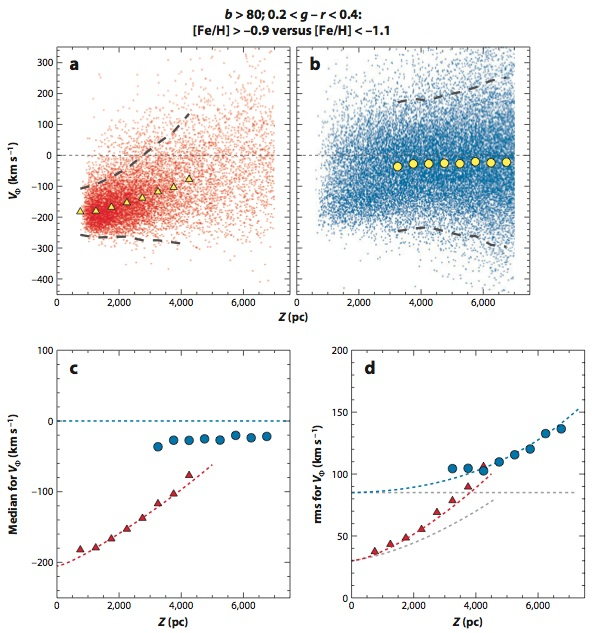
\includegraphics{figures/IBJ2012_fig7.jpg}}

{\bf Is velocity shear simply a consequence of thick disk 
becoming dominant over thin disk beyond 1-2 kpc?}


\end{center}
\end{minipage}

\begin{minipage}[t]{10cm}
\begin{center}
\vskip -1in
{\large \color{red} Disk vs. Halo Kinematics}
\end{center}

\begin{itemize}
\item {\bf Top panels:} small dots are individual stars, large symbols 
       are the median values.
\item {\bf \color{red} Top left:} disk stars show clear velocity shear
          (increase of $v_\Phi$ with $Z$)
\item {\bf \color{blue} Top right:} halo stars $<v_\Phi> \sim 220$ km/s
\item {\bf \color{red} Bottom left:} velocity shear is {\bf not} linear
\item {\bf \color{blue} Bottom right:} velocity dispersion slowly increases 
with $Z$ for disk stars, while for halo stars it is spatially invariant
\end{itemize}     

\end{minipage}}
\vfill 
\end{slide}
%------------------------------------------------------------------------------




 

%------------------------------------------------------------------------------
% TWO-SIDED PAGE 
\begin{slide}

{\bf Is velocity shear simply a consequence of thick disk 
becoming dominant over thin disk beyond 1-2 kpc?}


\scalebox{1.0}{\hskip -0.3in 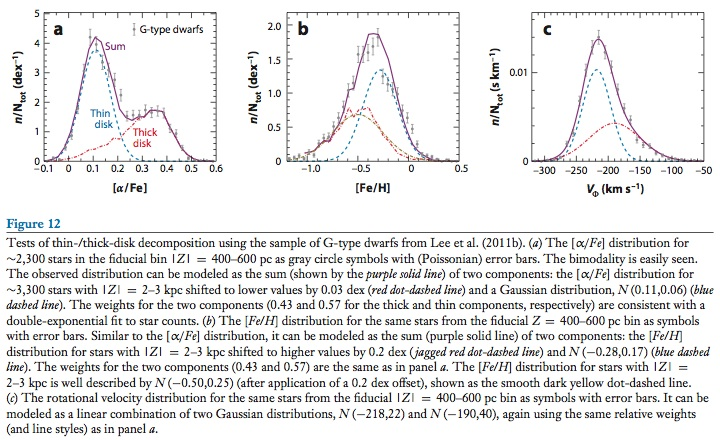
\includegraphics{figures/IBJ2012_fig12.jpg}}


\vfill 
\end{slide}
%------------------------------------------------------------------------------









%------------------------------------------------------------------------------
\begin{slide}
\begin{center}
{\large \color{red} 
                    The Local Mass Density   }
\end{center}

The $v_z$ Jeans equation (steady-state), see Lecture 7: 

\begin{eqnarray}
\color{blue} {\p(\nu \overline{v_R v_z}) \over \p R } + { \p (\nu \overline{v_z^2})
\over \p z } + { \nu \overline{v_R v_z} \over R} + \nu { \p \Phi \over
\p z} & = & 0. \nonumber
\end{eqnarray}

Drop the first and third terms because they are a factor of $\approx z^2/(RR_d)$
smaller than the second and fourth terms:

\eq{
 {1 \over \nu} { \p (\nu \overline{v_z^2}) \over \p z } = - { \p \Phi \over \p z} 
}

Near the plane of a highly flattened system, Poisson's equation becomes
\eq{
             { \p^2 \Phi \over \p z^2} = 4 \pi G \rho 
}



\vfill
\end{slide}



%------------------------------------------------------------------------------
\begin{slide}
\begin{center}
{\large \color{red} 
                    The Local Mass Density   }
\end{center}

\eq{
{ \p \over \p z } \left[{1 \over \nu} { \p (\nu \overline{v_z^2}) \over \p z } \right] = - 4 \pi G \rho 
}


If we can measure stellar counts ($\nu$) and velocity dispersion ($\overline{v_z^2}$) 
(as functions of $z$), then we can determine the local mass density $\rho$, which also 
includes the {\it dark matter} component, if any. This $\rho$ is called the Oort limit.

Oort (1932) estimated $\rho(R_\odot,z=0)$ = 0.15 M$_\odot$/pc$^3$.

Bahcall (1984) estimated $\rho(R_\odot,z=0)$ = $0.18\pm0.03$ M$_\odot$/pc$^3$.
This appeared as a significant result because {\color{blue} the local density of the luminous
matter (stars, gas and white dwarfs) is independently estimated at 0.11 M$_\odot$/pc$^3$,}
and thus suggests the existence of dark matter in the disk (the halo dark
matter contribution to local $\rho$ is less than 0.01 M$_\odot$/pc$^3$). 


However, Kuijken \& Gilmore (1989, MNRAS 239, 651) showed that previous samples and
analysis were flawed: {\color{red} there is no evidence that the dynamical
mass density is larger than the local density of the luminous
matter -- both are around 0.10 M$_\odot$/pc$^3$}. 

Bovy \& Tremaine (2012, ApJ 756, 89)  estimated local dark matter density as
\eq{
      \rho_{DM} = (0.008 \pm 0.003) \, M_\odot \, pc^{-3} \,\,\,\, (0.3\pm0.1 \, {\rm GeV cm}^{-3}) 
}
using disk star kinematics from SDSS (note the ten times better precision than in Bahcall's result). 

The Bovy \& Tremaine result represents a statistically significant (probably
the first one) dynamical detection of dark matter in the solar neighborhood!   

But note that it is only a $\sim$10\% effect (recall a factor of 3 effect from the Loebman et al. 2014 study). 


\vfill
\end{slide}
%------------------------------------------------------------------------------





%------------------------------------------------------------------------------
% TWO-SIDED PAGE 
\begin{slide}

\hbox to \hsize{
\begin{minipage}[t]{23cm}
\begin{center}
\vskip -1.2in 
{\large \color{red} Halo Velocity Ellipsoid Tilt}
\begin{itemize}
\item Three two-dimensional projections of the velocity distribution 
for two subsamples of candidate halo stars ($[Fe/H]<-1.1$) with 
$6<R/{\rm kpc}<11$, and {\color{red} $3<Z/{\rm kpc}<4$ (top)} \,\,\,\,\, and 
{\color{red} $-4<Z/{\rm kpc}<-3$ (bottom)}
\item {\color{blue} The $v_Z$ vs. $v_R$ velocity ellipsoid is aligned
with spherical coordinate system (Bond et al. 2010).} Confirms results of 
Smith et al. (2009) over 30 times larger area. 
\end{itemize}     

\vskip -3.95in
\scalebox{0.9}{\hskip -0.1in 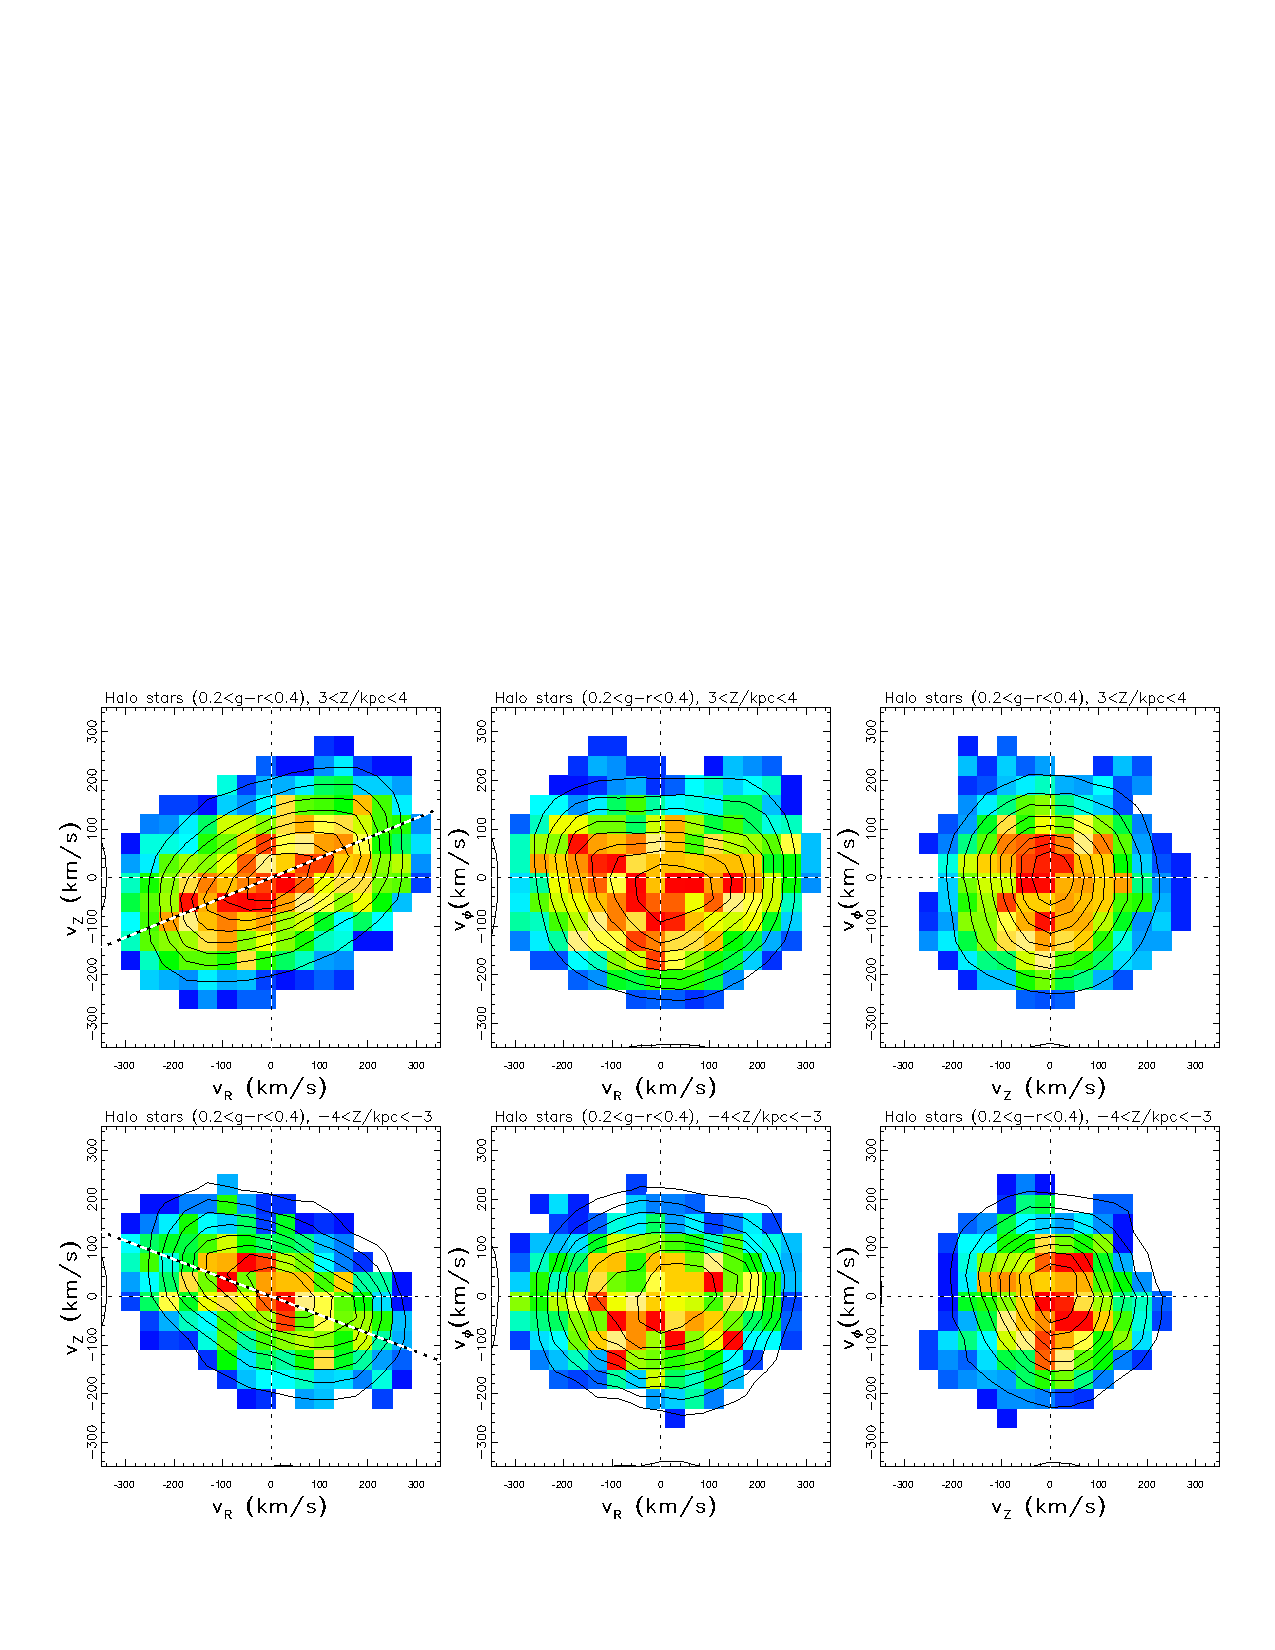
\includegraphics{figures/panelsVVmaps2_6D_HVT.pdf}}
\end{center}
\end{minipage}

\begin{minipage}[t]{0.01cm}
\begin{center}
\vskip -0.7in 
\end{center}

\end{minipage}}
\vfill 
\end{slide}
%------------------------------------------------------------------------------




%------------------------------------------------------------------------------
% TWO-SIDED PAGE 
\begin{slide}

\hbox to \hsize{
\begin{minipage}[t]{13cm}
\begin{center}
\vskip -0.5in
\scalebox{0.7}{\hskip -1.5in 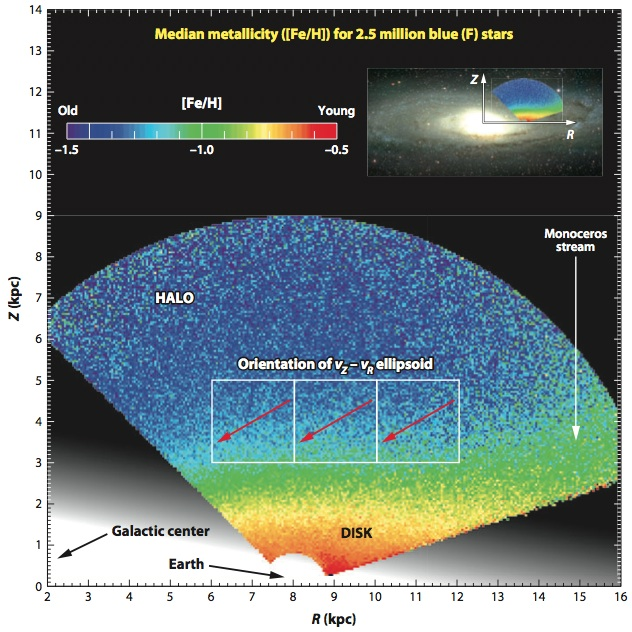
\includegraphics{figures/IBJ2012_fig5.jpg}}

{\bf A comparison of counts, metallicity distribution and kinematics.} 


\end{center}
\end{minipage}

\begin{minipage}[t]{10cm}
\begin{center}
\vskip -1in
\end{center}

\begin{itemize}
\item 
{\large The arrows illustrate the variation of the ellipsoid orientation, 
which {\color{red} always points toward the Galactic center!}}
\item This measurement can be used to infer the shape of gravitational
potential (Loebman et al. 2012, ApJ 758, L23, see Lecture 10). 
\end{itemize}     

\end{minipage}}
\vfill 
\end{slide}
%------------------------------------------------------------------------------


%------------------------------------------------------------------------------
% TWO-SIDED PAGE 
\begin{slide}

\hbox to \hsize{
\begin{minipage}[t]{23cm}
\begin{center}
\vskip -1.2in 
{\large \color{red} A smooth global kinematic model is possible...}
\begin{itemize}
\item Overall kinematic behavior can be captured by a simple model
\end{itemize}     

\vskip 0.31in
\scalebox{0.8}{\hskip -0.1in 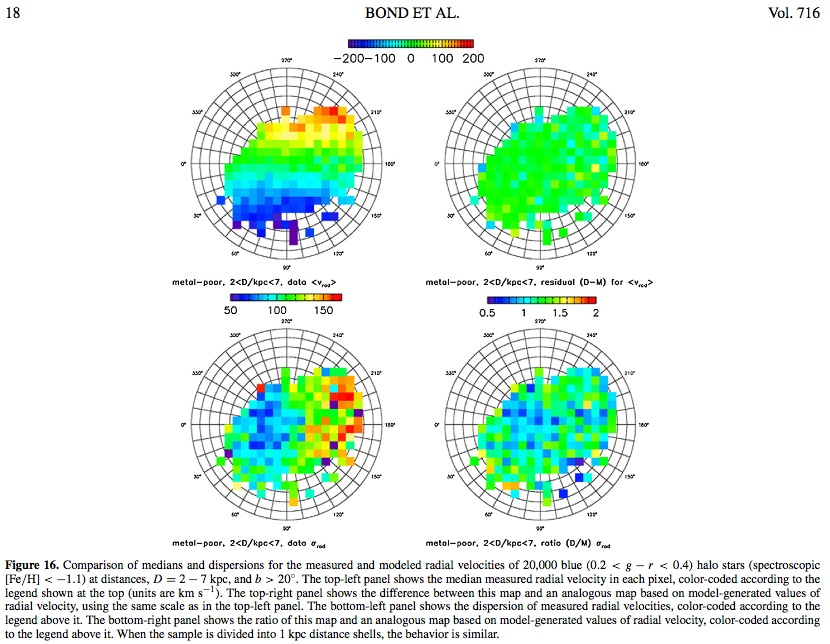
\includegraphics{figures/BondFig2.jpg}}
\end{center}
\end{minipage}

\begin{minipage}[t]{0.01cm}
\begin{center}
\vskip -0.7in 
\end{center}

\end{minipage}}
\vfill 
\end{slide}
%------------------------------------------------------------------------------



%------------------------------------------------------------------------------
% TWO-SIDED PAGE 
\begin{slide}

\hbox to \hsize{
\begin{minipage}[t]{23cm}
\begin{center}
\vskip -1.2in 
{\large \color{red} A smooth global kinematic model is possible...}
\begin{itemize}
\item for both low- and high-metallicity components
\end{itemize}     

\vskip 0.31in
\scalebox{0.8}{\hskip -0.1in 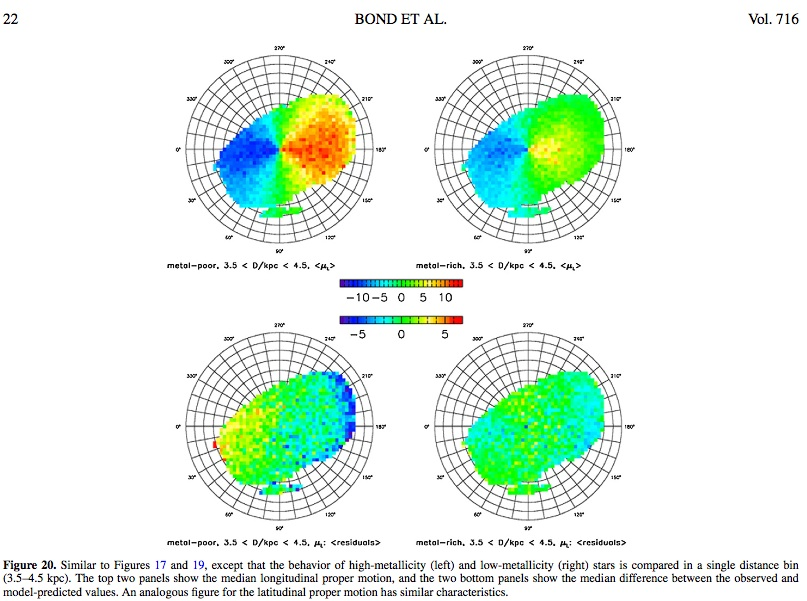
\includegraphics{figures/BondFig3.jpg}}
\end{center}
\end{minipage}

\begin{minipage}[t]{0.01cm}
\begin{center}
\vskip -0.7in 
\end{center}

\end{minipage}}
\vfill 
\end{slide}
%------------------------------------------------------------------------------

%------------------------------------------------------------------------------
% TWO-SIDED PAGE 
\begin{slide}

\hbox to \hsize{
\begin{minipage}[t]{23cm}
\begin{center}
\vskip -1.2in 
{\large \color{red} Empirical Model for Mock Catalogs: {\bf Galfast}}
\begin{itemize}
\item Web service by Mario Juri\'{c} based on smooth spatial, metallicity 
and kinematics distributions measured by SDSS
\item Available from www.mwscience.net/galfast
\item A valuable tool when searching for substructure in data, or
      comparing to theoretical models
\item For example, can easily make mock catalogs for surveys such
      as SDSS, SkyMapper, Pan-STARRS, Gaia, and LSST 
\item Additional very popular codes: Besancon and Trilegal. 
\end{itemize}     

\vskip -3.0in
\scalebox{1.0}{\hskip -0.1in 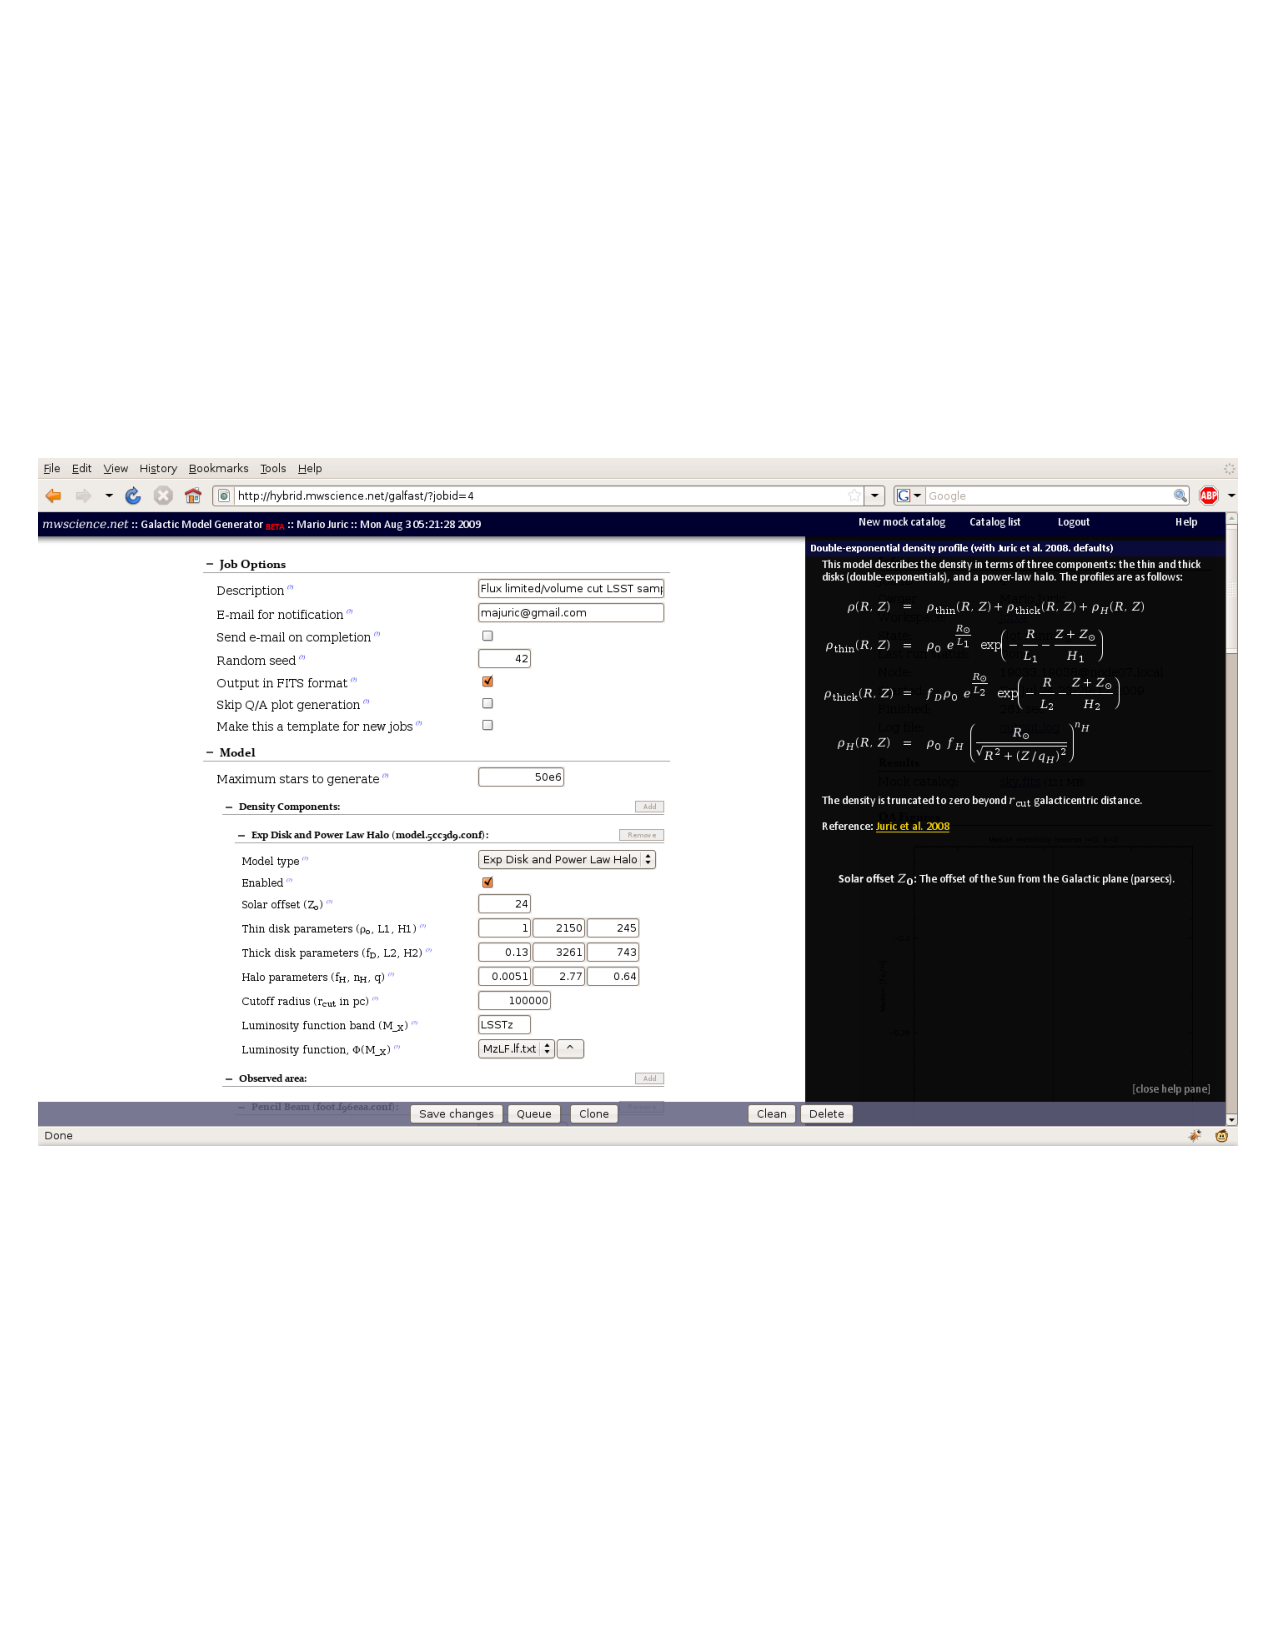
\includegraphics{figures/galfast1.pdf}}
\end{center}
\end{minipage}

\begin{minipage}[t]{0.01cm}
\begin{center}
\vskip -0.7in 
\end{center}

\end{minipage}}
\vfill 
\end{slide}
%------------------------------------------------------------------------------






%------------------------------------------------------------------------------

\begin{slide}

\begin{center}
\bfseries
\large \colour{red} Summary of Metallicity/Kinematics Results
\end{center}
\vskip 0.2in
\begin{itemize}
   \item {\color{blue} Clumps/overdensities/streams are an integral part of
       Milky Way structure,} both for halo and disk components;  
       the kinematics and metallicity distributions are exceedingly complex.
  \item 
    {\color{blue} Nevertheless, it is possible to construct a reasonably good
   model for the smooth global behavior (Bond et al. 2010)}
   \item The rotational lag (velocity shear) and metallicity distribution
     for disk stars are {\color{blue} smooth} functions of $Z$
   \item The halo velocity ellipsoid is invariant in spherical coordinates (within 10 kpc or so). 
\end{itemize}    

{\colour{blue} SDSS has revolutionized studies of the Galactic structure;}

{\colour{red} Gaia and LSST will do even better!} (the last lecture)

\end{slide}



%------------------------------------------------------------------------------




\end{document}



